\section{Choice of methods}
\lb{sec:methods}

\subsection{General methodology}

The first choice one has to make in constructing a probabilistic catalog is the input data and the machine learning methods.
For the input data we take associated point sources (PS) in the 3FGL or 4FGL-DR2 catalogs, which we split into training and testing subsets.
We consider four machine learning algorithms: random forests \citep[RF,][]{709601, Breiman:2001hzm}, 
boosted decision trees \citep[BDT,][]{friedman2001},  
logistic regression \citep[LR,][]{cox1958}, 
and neural networks \citep[NN,][]{Hopfield:1982pe}.
Although the performance of algorithms on testing data is slightly different, 
we report the classification probabilities for all four algorithms.
The difference among the predictions will serve as a measure of modeling uncertainty related 
to the choice of the classification algorithm.

\subsection{Discussion of the choice of the classification algorithms}
\lb{sec:class_alg}


One of the most simple and transparent algorithms for classification is decision trees.
In this algorithm, at each step the sample is split into two subsets using one of the input features.
The choice of the feature and the separating value are determined by minimizing an objective function, such as misclassification
error, Gini index, or cross-entropy.
This method is very intuitive, since at each step the results can be described in words, 
for example, at the first step, the sources can be split in mostly Galactic and extragalactic by a cut on the Galactic latitude.
At the next step, the high latitude sources can be further subsplit into millisecond pulsars and other sources, by a cut on the spectral index around 1 GeV (pulsars have a hard spectrum below a few GeV) etc.
One of the problems with decision trees is either overfitting or bias: if a tree is too deep, then it will pick up particular cases of the training sample resulting in overfitting, while too shallow trees would not be able to describe the data well, which can lead to bias. 
As a result, one needs to be very careful in selecting the depth of the tree.
This problem can be avoided if a random subset of features is used to find a division at each node. This is the basis of the RF algorithm,
where the final classification is given by an average of several trees with random subsets of features used at each node.
Another problem with the simple trees is that it can miss the classification of some subsets of data. In BDT algorithms, the final classification is given by a collection of trees, where each new tree is created by increasing the weights of misclassified samples of the previous step. 
Finally, simple trees predict classes for the data samples, while we would like to have probabilities of classes (also known as soft classification).
RF and BDT algorithms, by virtue of averaging, provide probabilities. As a result, we will use RF and BDT algorithms rather than simple decision trees in this paper.

Tree-based algorithms, even after averaging in RF and BDT methods, have sharp edges among domains with different probabilities.
In LR algorithm, the probabilities of classes are by construction smooth functions of features.
In particular, for two-class classification the probability of class 1, given the set of features $x$, is modeled by sigmoid (logit) function
\bea
\lb{eq:logit}
p_1(x) = \frac{e^{m(x)}}{1 + e^{m(x)}}.
\eea
The probability of class 0 is then modeled as $p_0(x) = 1 - p_1(x)$.
If $m(x)$ is a linear function of features, then the boundary between the domains, defined, e.g., as $p_1(x) = 0.5$, will be linear
at $m(x) = 0$.
More complicated boundaries can be modeled by taking non-linear functions $m(x)$.
Unknown parameters of the function $m(x)$ are determined by maximizing the log likelihood of the model given the known classes of the data in the training sample.
A useful feature of the LR method is that it, by construction, provides probabilities of classes with smooth transitions among domains of different classes.
A limitation is that the form of the probability function is fixed to the sigmoid function in Eq. (\ref{eq:logit}).

We notice that if $m(x)$ is a linear function of features $x$, then the LR model is obtained by an application of sigmoid function to a linear combination of input features.
This is in fact a single layer perceptron, or a NN, with several input nodes (each node corresponds to a feature) and one output node, which corresponds to $p_0(x)$, but without any hidden layers.
The output value is obtained by a non-linear transformation (sigmoid) of a linear combination of features.
Neural network with several hidden layers is obtained by a sequence of non-linear transformations of linear combinations of features.
In particular, the values in the first hidden layer are obtained by a non-linear transformation of linear combinations of input features.
Then the values in the second hidden layer are obtained by a non-linear transformation of linear combinations of values in the first hidden layer etc.
In the context of neural networks, the non-linear transformations are called activation functions.
If the activation function for the output layer is sigmoid, then the output value (values) can be interpreted as probabilities.


\section{Construction of probabilistic catalogs}
\lb{sec:training}

One of the first problems, one has to deal with for the 3FGL and 4FGL-DR2 catalogs, is that
some of the sources in the catalogs have missing or unphysical values (e.g., infinity).
In order to avoid a bias in predictions, we include sources with missing or unphysical values only in testing or in predictions (for unassociated sources), but not in training.
If the value is infinity, then we formally substitute it by the largest value found in the samples multiplied by 10.
An unphysical zero (e.g., in significance) is substituted by the smallest value in the sample divided by 10,
while a missing value is substituted by the average in the sample.
There can be other ways to replace the missing or unphysical values, e.g., by using k nearest neighbors regression, 
but since the number of such sources is relatively small (13 for 3FGL and 14 for 4FGL-DR2), 
the choice of the method to replace the missing values does not significantly affect the results.
In the final probabilistic catalogs, we use a column ``Missing\_Values\_Flag'' to mark sources with missing or unphysical values.

As an example of the construction of a probabilistic catalog, we will use the 3FGL catalog.
In this section we will perform a two-class classification to separate PS into pulsars and AGNs.
Thus for training and testing, we subselect the sources, which are associated to pulsars and AGNs.
The three-class classification into pulsars, AGNs, and other sources is discussed in Section \ref{sec:3class}.
After the training of the algorithms, we test the performance with the test sources and predict the classes of unassociated sources.
The general workflow will have the following steps:
\ben
\item
Select data for learning and testing.
\item
Optimize algorithms using training datasets.
We select meta-parameters of the algorithms by optimizing accuracy of classification and test for overfitting using the test datasets.
In order to get stable results, we repeat the separation of the data into training and testing samples 100 times and 
average the accuracy.
\item
Make prediction for unassociated point sources of the 3FGL.
We also apply the classification for associated sources, which we use for consistency checks.
\een
As a result of the analysis in this section, we select meta-parameters for the four ML algorithms,
which we use in the following section for a construction of probabilistic catalogs
based on the \Fermi-LAT 3FGL and 4FGL-DR2 catalogs.



\subsection{Data and feature selection}

For training of the algorithms we use the associated sources without missing or unphysical values, 
which were classified as either AGNs (classification labels in the 3FGL catalog: agn, FSRQ, fsrq, BLL, bll, BCU, bcu, RDG, rdg, NLSY1, nlsy1, ssrq, and sey) or pulsars (classification labels in 3FGL: PSR, psr). 
There are 1905 such sources in the 3FGL catalog. 


There are several tens of features of point sources quoted in the catalog, such as the position, photon and energy fluxes integrated in different energy bands, spectral parameters, variability index as well as corresponding uncertainties. 
We took the main features and calculated their Pearson correlation coefficients. 
A graphical representation of the correlation table is shown in Fig.~\ref{fig:assoc_corr_3fgli}. 
In the following, if two features have (anti)correlation $\gtrsim 0.75$ 
($\lesssim -0.75$), then we keep only one of the features for classification.
Along with the normal features we also add 4 hardness ratios defined as $hr_{ij} = \frac{EF_j - EF_i}{EF_j + EF_i}$, where $EF_i$ is the energy flux in bin $i$
and $j = i + 1$ (i.e., the bins are consecutive).
We have added the hardness ratios in order to allow the algorithms to ``construct'' their own features from the raw data rather than to use the 
derived features, such as 500MeV\_Index or integrated energy flux.

\begin{figure}[h]
\centering
\hspace*{-0.9cm}
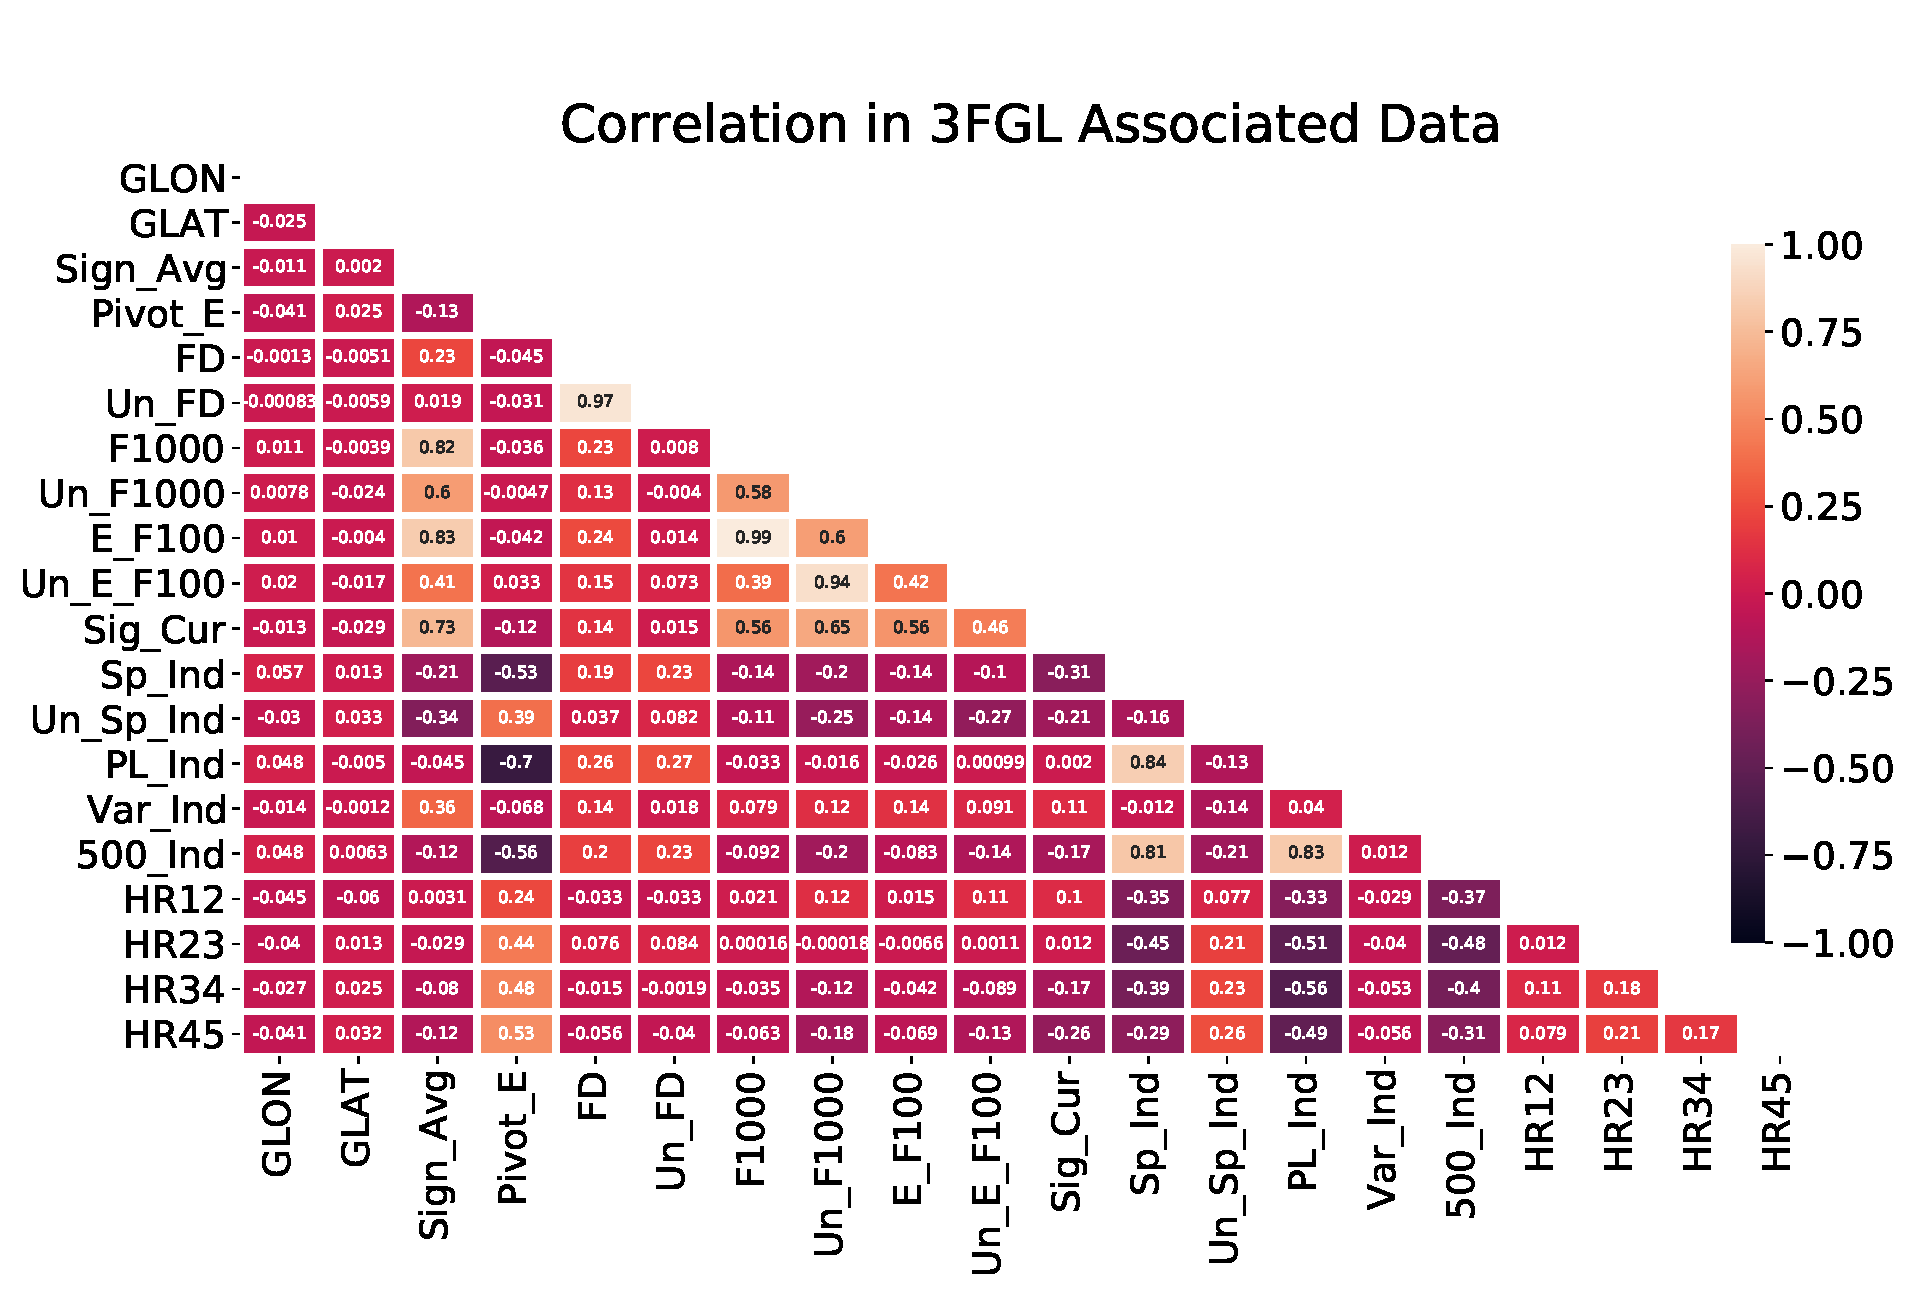
\includegraphics[width=0.55\textwidth]{plots/new_correlations.pdf}
\caption{The corelation matrix of features for 3FGL associated sources.
The ``500MeV\_Index'' is defined in Eq. (\ref{eq:n500_def}), all other features are taken directly 
from the 3FGL catalog.
}
\label{fig:assoc_corr_3fgli}
\end{figure}

Spectral index is one of the important characteristics of sources. 
Unfortunately in the 3FGL catalog, the definition of the spectral index is different for associated and unassociated sources.
In particular, the gamma-ray flux of pulsars is described by a power-law with a (super)exponential cutoff $\propto E^{-\Gamma} e^{-(E / E_c)^b}$ 
function, where the ``Spectral\_Index'' feature in the catalog is the parameter $\Gamma$.
Gamma-ray flux of unassociated sources with significant curvature is represented by log-parabola function $\propto (E/E_0)^{-\al - \bt \ln (E/E_0)}$,
where the ``Spectral\_Index'' feature is the parameter $\al$, i.e., the tilt in the spectrum at the pivot energy $E_0$ (which also varies for different sources).
Since the ``Spectral\_Index'' feature has different definitions for associated pulsars and for possible pulsars among unassociated sources,
its use for training the algorithms to separate pulsars from AGNs is problematic.
If one fits all spectra of sources in the catalog by a power-law function, then the corresponding indices of the power laws are represented by
``PowerLaw\_Index'' feature in the catalog.
This feature is defined uniformly for all associated and unassociated sources, i.e., it is safe to use for training.
Unfortunately, the power-law function is not a good description of the gamma-ray flux from pulsars.
Consequently, in the classification of the 3FGL sources we have constructed a new feature: the index at 500 MeV (denoted in the following as ``500MeV\_Index''), defined as minus the derivative of the log flux:
\bea
\lb{eq:n500_def}
n({\rm 500\,MeV}) = - \left. \frac{d \ln F}{d \ln E} \right|_{E = \rm 500\,MeV}
\eea
For log parabola and for power law with (super)exponential cutoff it is respectively
\bea
n(\rm 500\,MeV) &=& \al + 2 \bt \ln(\rm 500\,MeV / E_0)    \\
n({\rm 500\,MeV}) &=& \Gamma + b\,({\rm 500\,MeV} / E_c)^b
\eea
This feature has a more uniform definition for all sources in the 3FGL catalog than the Spectral\_Index. It also has a better separating power 
than PowerLaw\_Index, provided that pulsars have typically harder spectra at energies below 1 GeV than AGNs.

Taking into account the correlation among the features and the above discussion of the spectral index definition,
we have selected the following eleven features for the classification of the 3FGL sources:
Galactic latitude (GLAT), Galactic longitude (GLON), ln(Energy\_Flux\_100), $\ln$(Unc\_Energy\_Flux100), 500MeV\_Index, $\ln$(Signif\_Curve), 
$\ln$(Variability\_Index), and four hardness ratios $HR_ij$.  
The table of features and their statistics can be found in Appendix \ref{sec:app}.






\subsection{Construction of classification algorithms}

The number of tunable parameters in the classification algorithms is not fixed a priori. 
Moreover there is a certain freedom in the choice of the architecture of the algorithms, such as
the number of hidden layers and the number of neurons in neural networks.
In general, one starts with a simple model and increases the complexity (the number of tunable parameters)
until the model can describe the data well, but does not overfit it.
The overfitting is tested by splitting the input data into the training and testing samples.
The training sample is used for optimizing the parameters,
while the test sample is used to check that the model is not overtrained (for overtrained models the accuracy on the test
sample is significantly worse than the performance on the training sample).
We will split the data randomly into 70\% training and 30\% testing samples.



\subsubsection{Random Forests}
\lb{sec:rf}

The two main parameters characterizing the RF algorithm are the number of trees and the maximum depth allowed in the trees. 
We use the Gini index as the objective function for the optimization of parameters (split values of features in the nodes).

\begin{figure}[h]
\centering
\hspace*{-0.5cm}
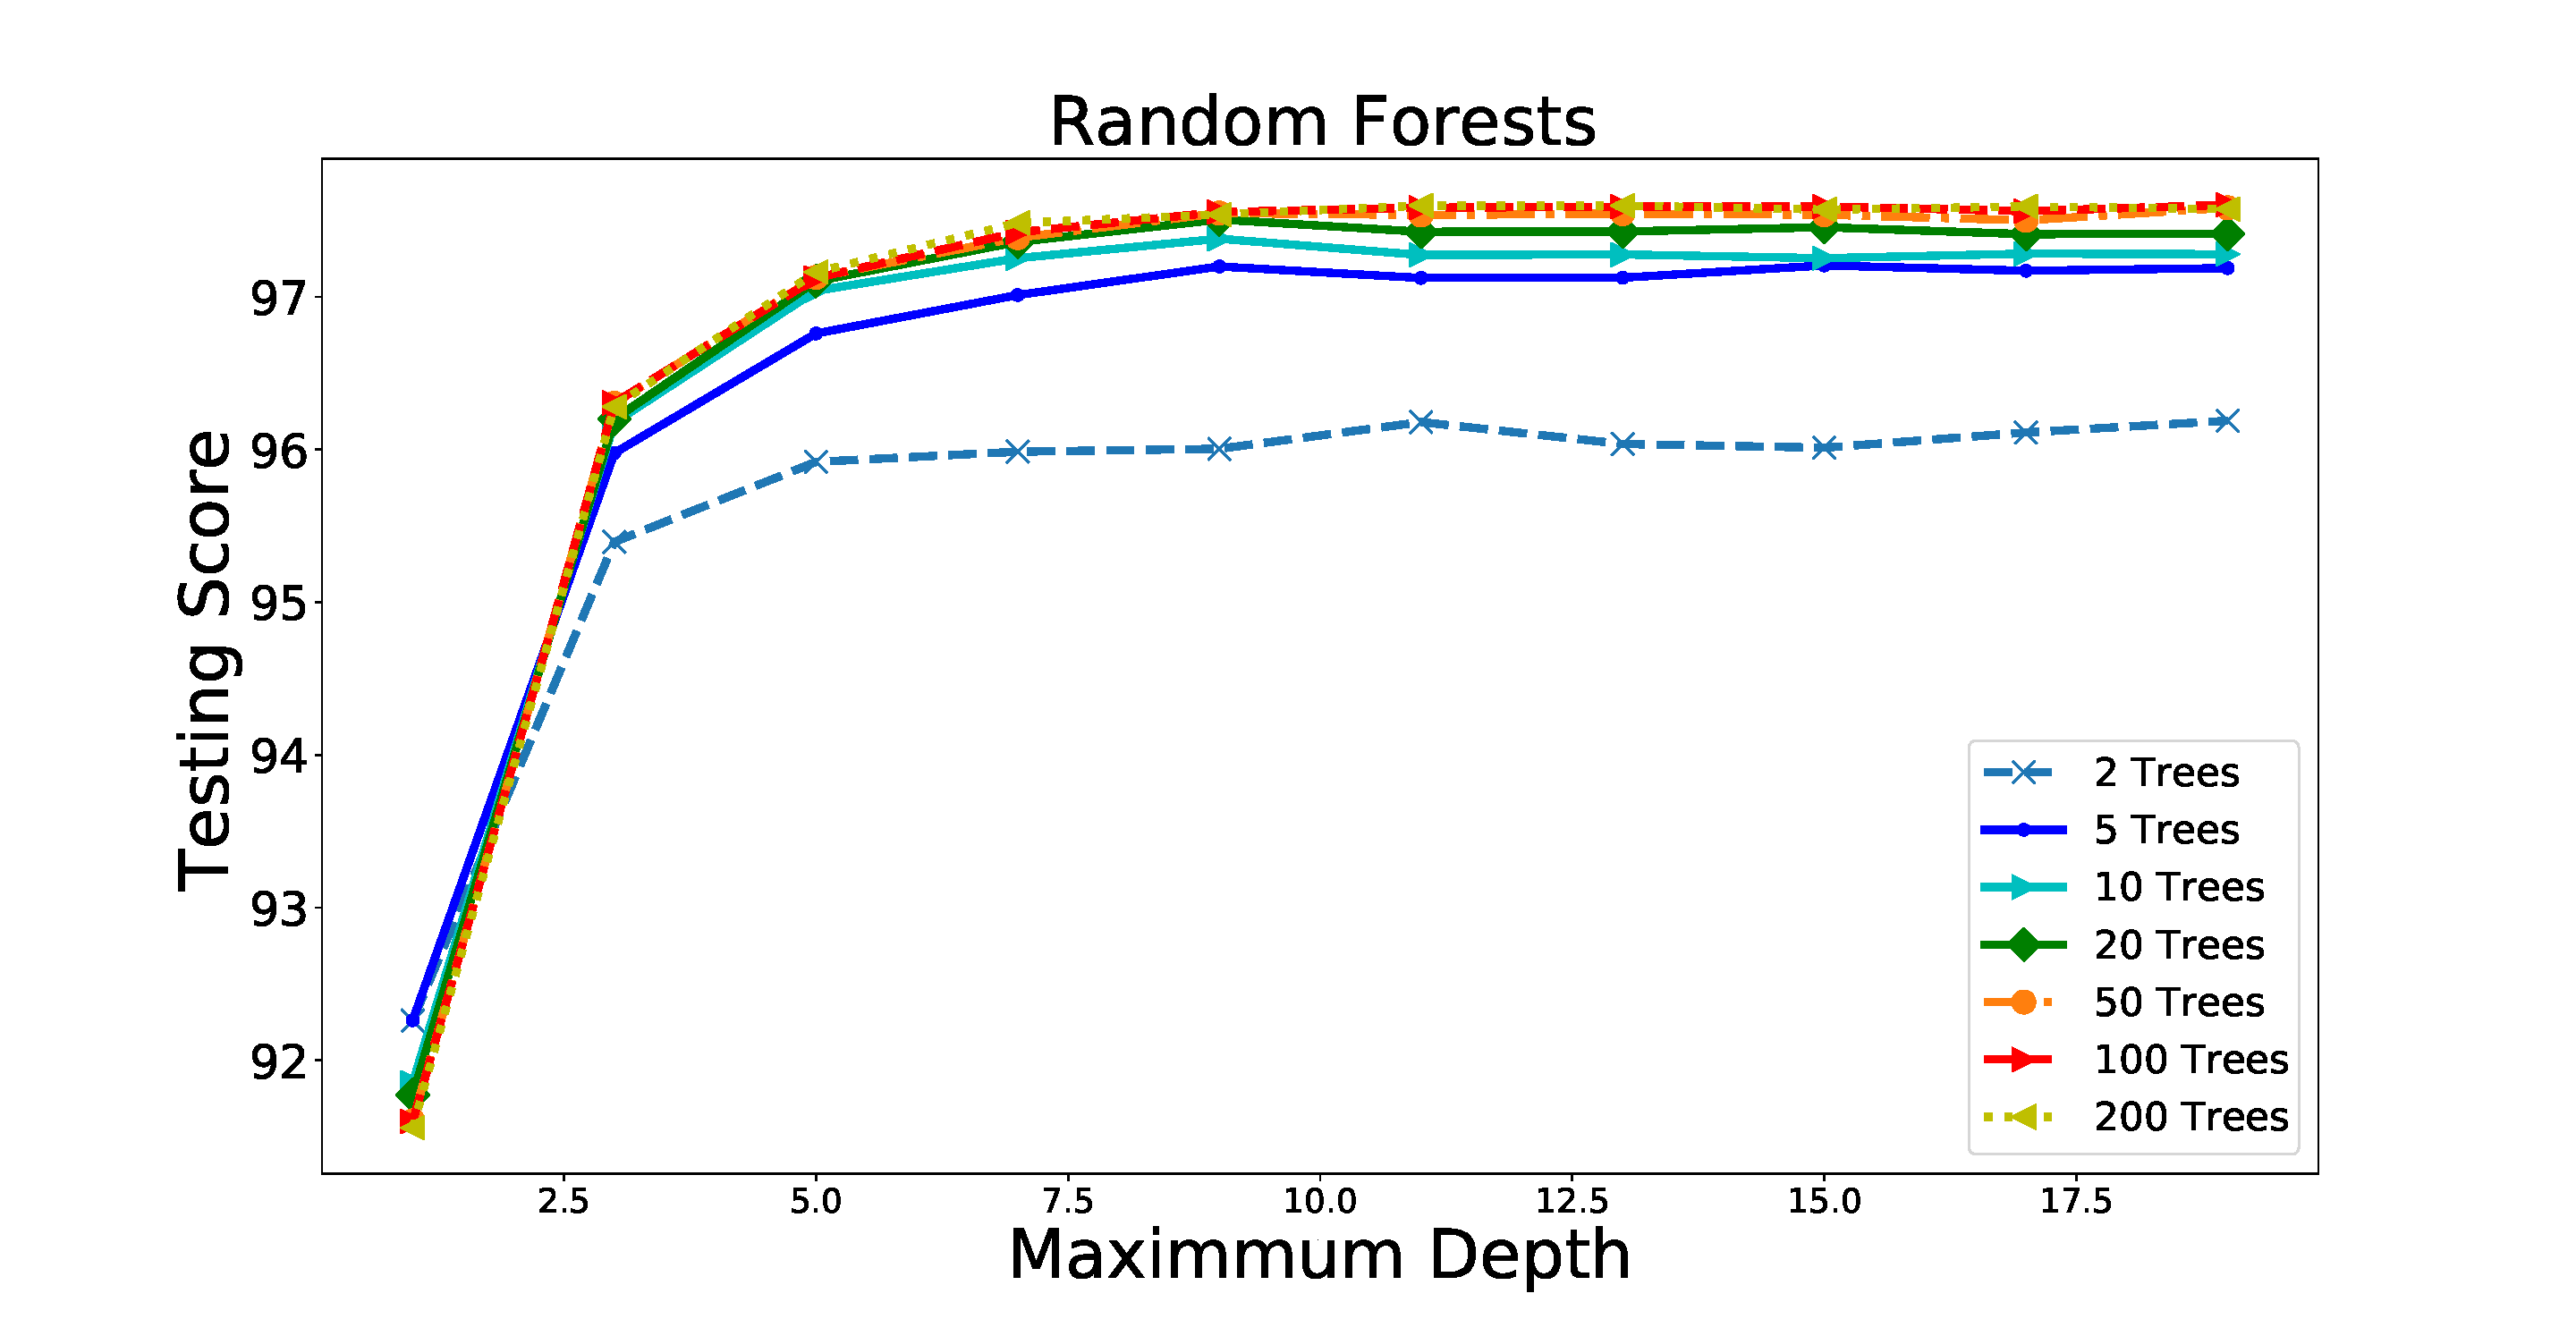
\includegraphics[width=0.5\textwidth]{plots/rf_train_assocnewfeats.pdf}
\caption{
Test score (accuracy) of RF classification as a function of the number of trees and 
the maximal depth of trees.
}
\label{fig:RF_complexity}
\end{figure}

Fig. \ref{fig:RF_complexity} shows the dependence of the accuracy of the test sample as a function of maximum depth and the number of trees. 
The results for each point are averaged over 100 realizations of the split into training and testing samples.
We notice that the accuracy does not decrease as the maximal depth of the trees increases, i.e., there is no overfitting as the complexity of the model increases with increased maximum depth.

This is due to the random choice of a subset of features at each node (maximal number of allowed features is $\sqrt{\text{\# features}}$).
It is also insensitive to the number of trees above approximately 20 trees.
For classification we will use 50 trees with the maximum depth of 6.


In order to illustrate the separation of PS into AGNs and pulsars, we retrain the RF algorithm using only two features: log of curvature significance and log of the variability index, and plot the resulting probabilities of classes in Fig. \ref{fig:RF_domains}
for the model with 50 trees with the maximum depth of 6.
The probabilities are averaged over 100 splits into training and testing samples.
It is important to note that in this plot the model is trained on only two features. Nevertheless a good testing accuracy of 97\% is reached, 
which is similar to the accuracy of the RF classification with all 11 features.
For the final classification with RF, we use 11 features and average over 1000 splits into training and testing samples.

\begin{figure}[h]
\centering
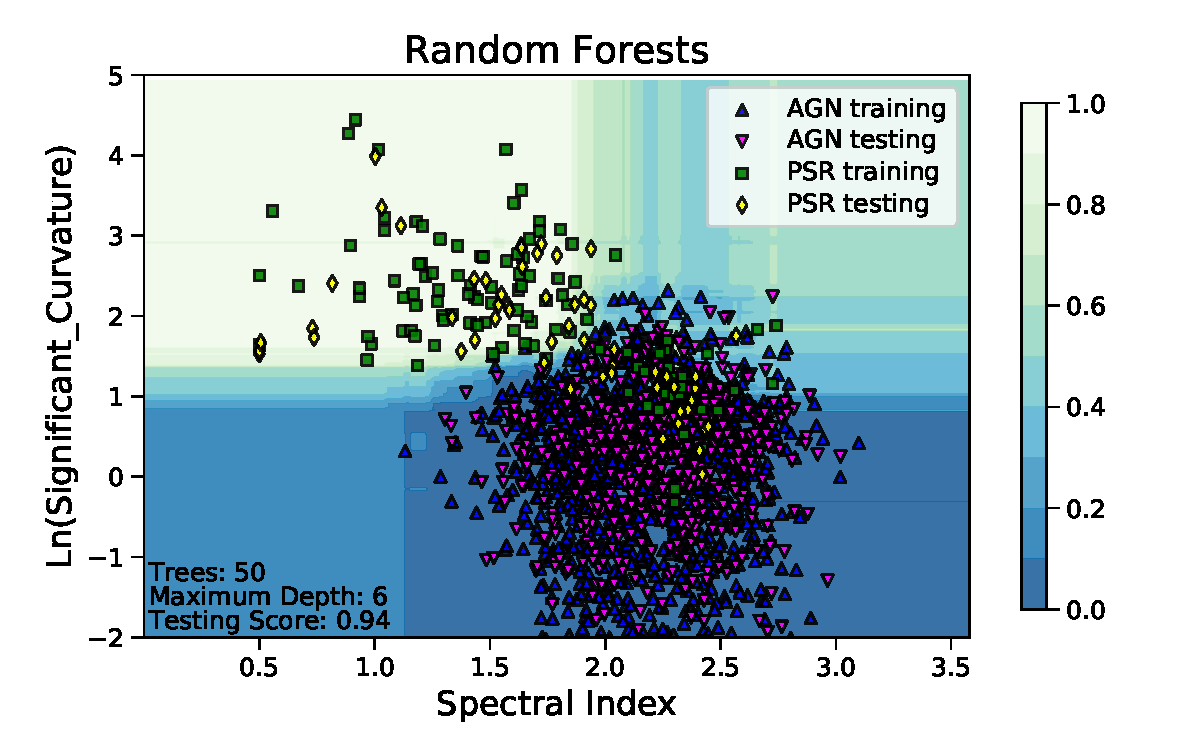
\includegraphics[width=0.5\textwidth]{plots/classification_domains/rf_50_6_final.pdf}
\caption{RF classification domains showing class probabilities for training with two features
averaged over 100 random splits into training and testing samples.
One of these splits is shown for illustration.
Color scale describes the probability for a source to be a pulsar.
}
\label{fig:RF_domains}
\end{figure}



\subsubsection{Boosted Decision Trees}

The meta-parameters for BDT algorithms are similar to RF algorithms: they are the number of trees and the maximal depth.
We used the Gradient Boosting algorithm for the construction of BDT \citep{gb}.
The classification is performed by a weighted average of trees, where the trees are constructed recursively in order to better address 
misclassifications from the previous step. 
Dependence of the accuracy on tree depth is shown in Fig.~\ref{fig:BDT_depth}. 
Unlike the RF, which is also an ensemble based method, the testing accuracy drops for the maximal depths larger than 7. 


\begin{figure}[h]
\centering
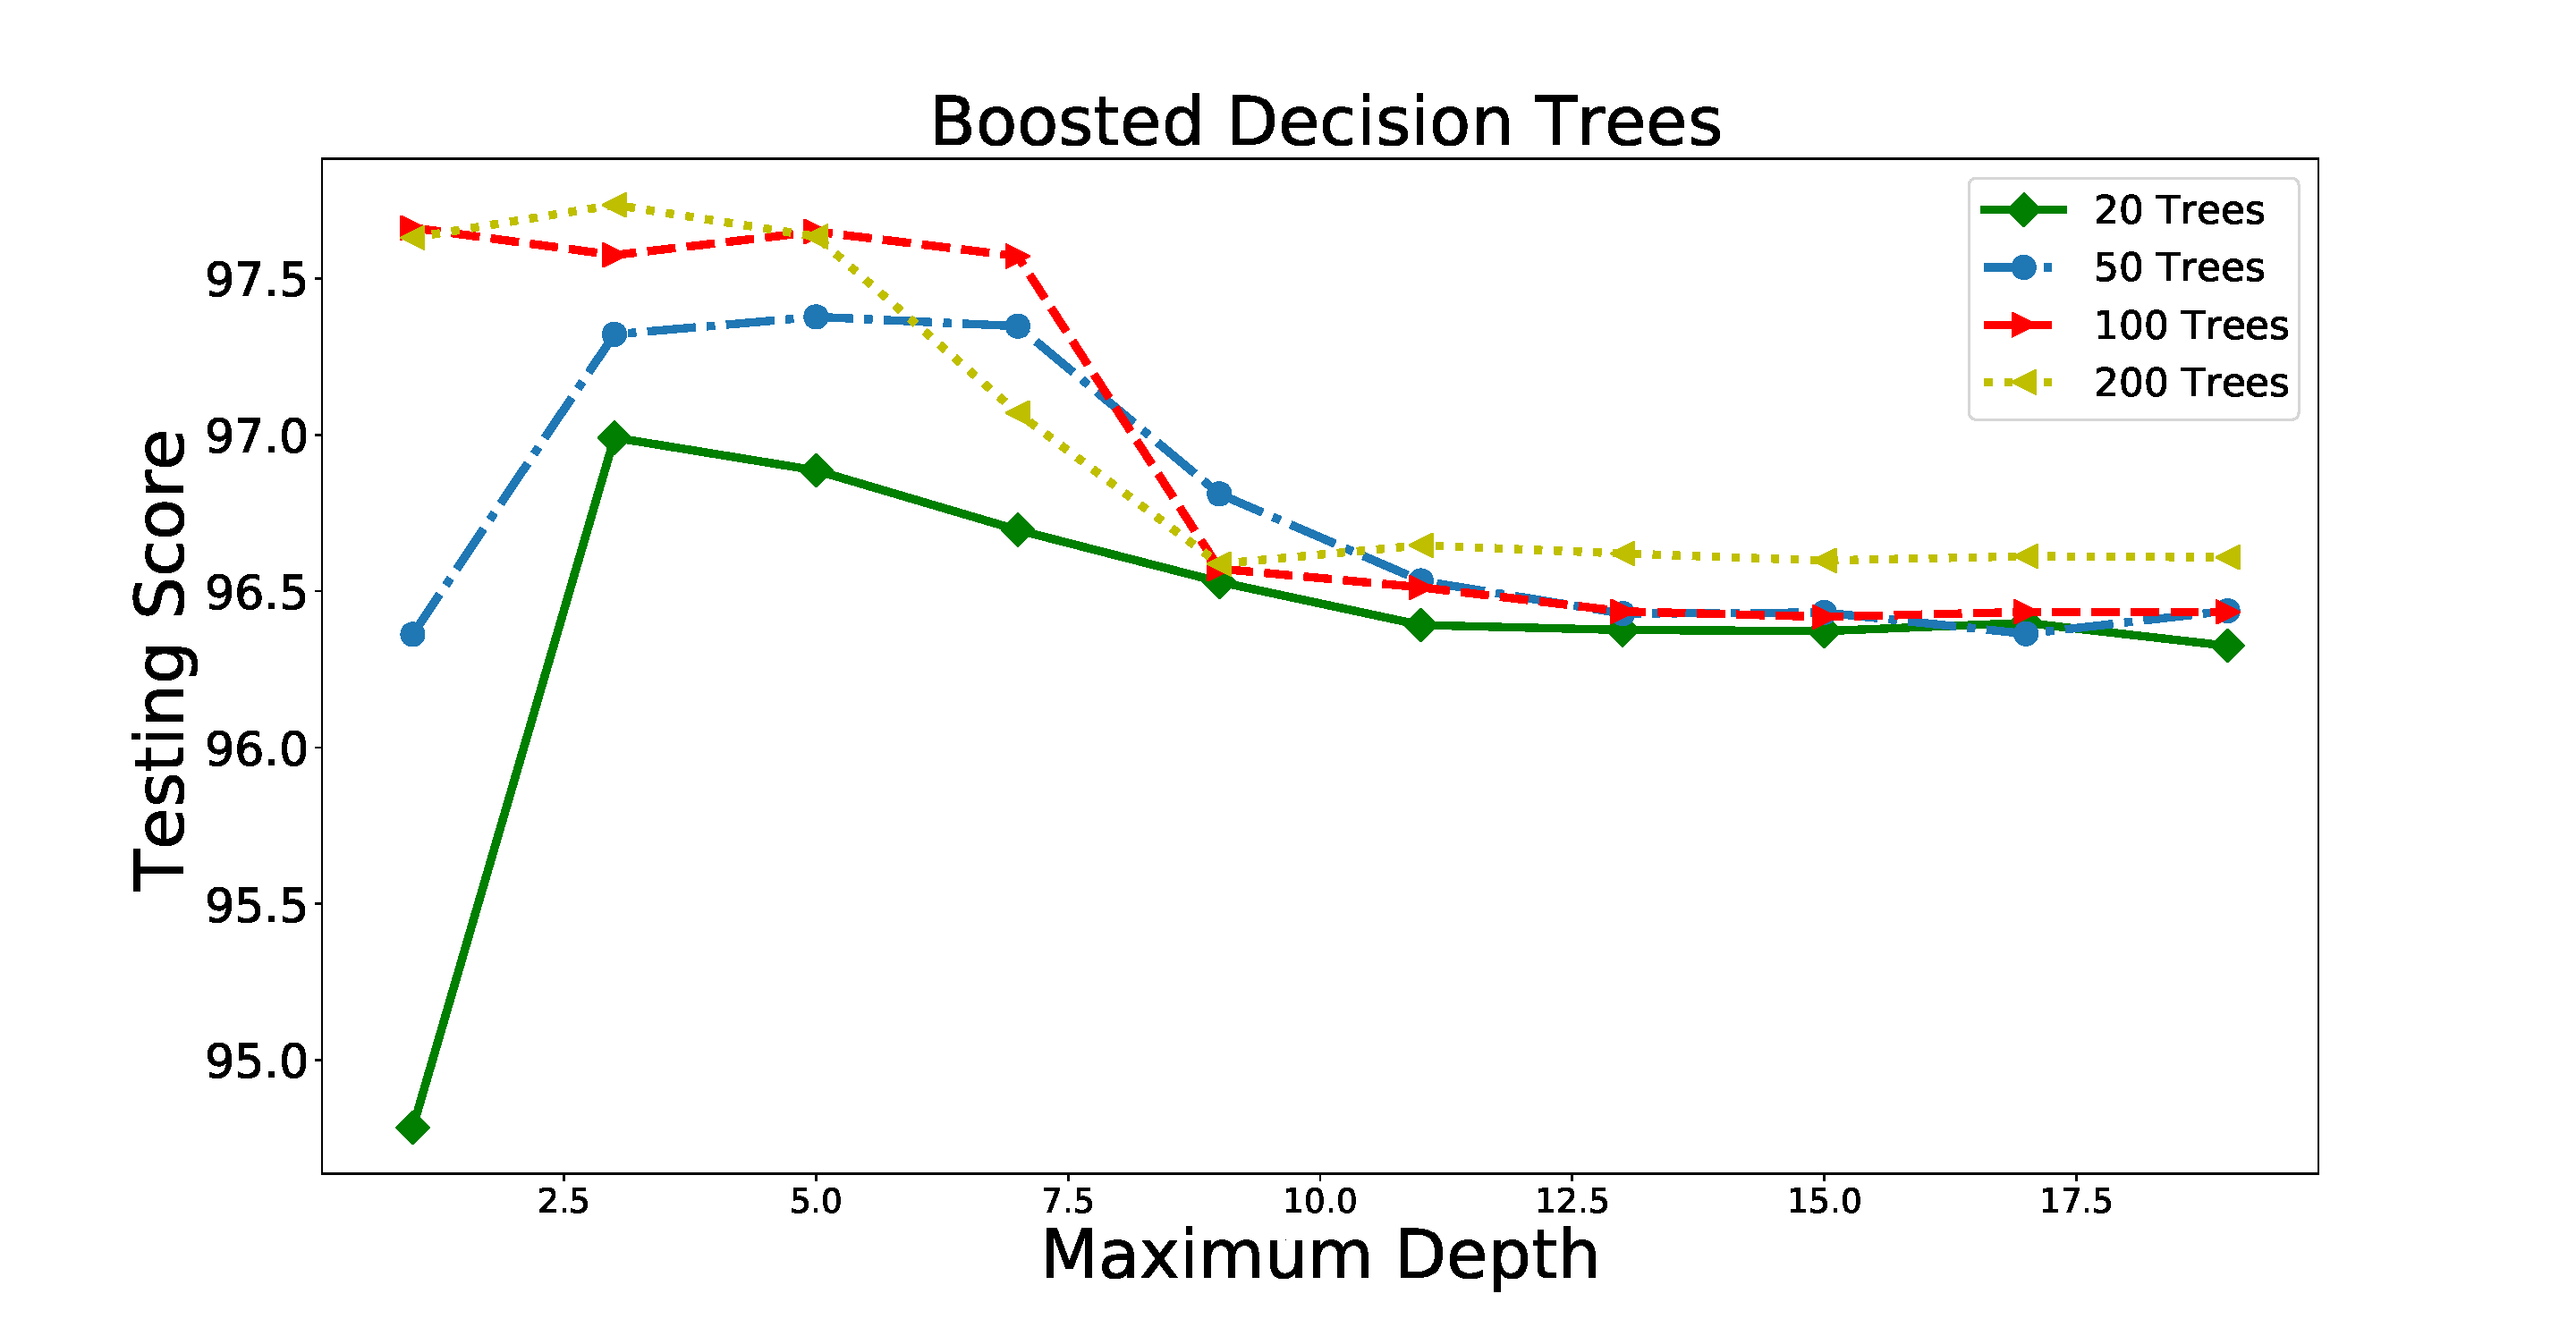
\includegraphics[width=\twopicsp\textwidth]{plots/bdt_train_assocnewfeats.pdf}
\caption{Dependence of BDT accuracy on maximum depth and the numbers of trees.}
\label{fig:BDT_depth}
\end{figure}

The classification domains in case of two features for 20 trees and the maximum depth of 2 is presented in Fig.~\ref{fig:BDT_domains}. 
For the classification we will use BDT with 100 trees and the maximum depth of 2.


\begin{figure}[h]
\centering
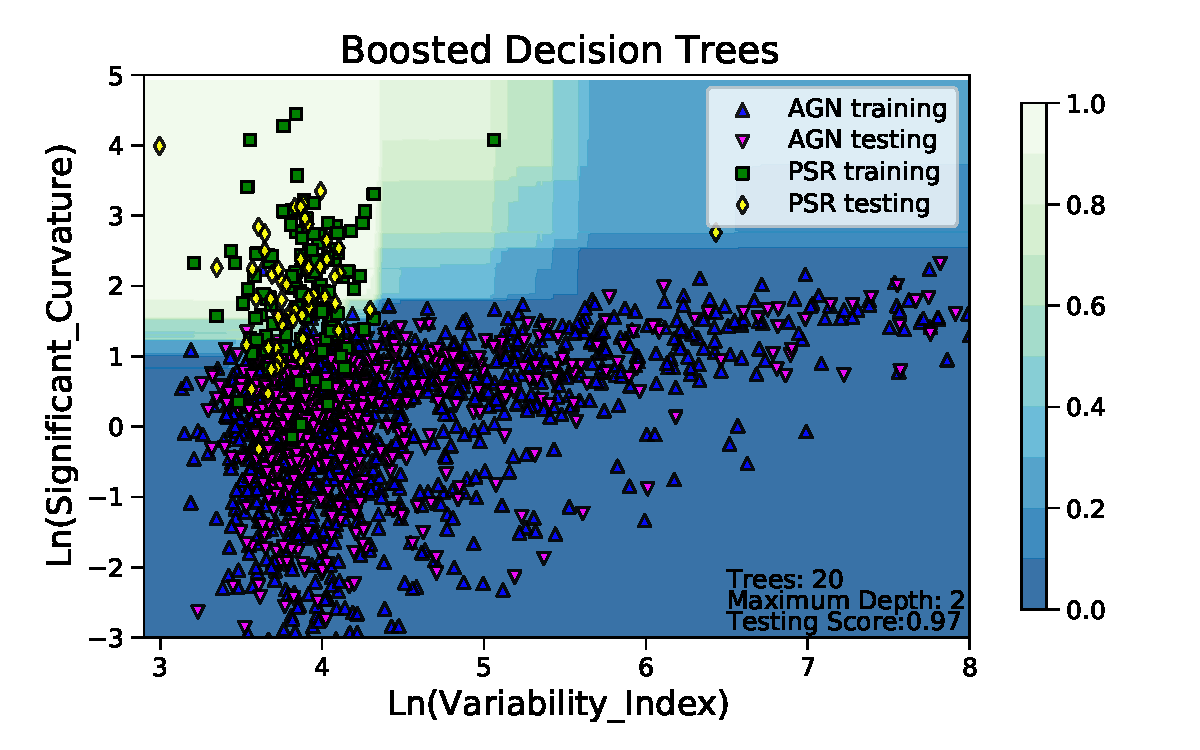
\includegraphics[width=0.5\textwidth]{plots/classification_domains/bdt_20_2.pdf}
\caption{Classification domains for BDT for training with two features 
averaged over 100 splits into training and testing samples.
}
\label{fig:BDT_domains}
\end{figure}



In tree-based algorithms, one can calculate feature importance by using the averaged reduction of impurity for nodes (Gini index in our case) involving the different features. 
The importance of features for the case of two different algorithms: RF with 50 trees and maximum depth of 6, and BDT with 100 trees with maximum depth of 2,  are shown in Table \ref{tab:feat_imp}.
We find that the most important feature for both cases is the significance of curvature.
Other significant features are the hardness ratio of the last two energy bins, uncertainty of the energy flux at 100 MeV, and the variability index.


\begin{table}[!h]
\tiny
\centering
\renewcommand{\tabcolsep}{1mm}
\renewcommand{\arraystretch}{1}

\begin{tabular}{c c c}
\hline
\hline
Feature & RF: 50, 6 & BDT: 100, 2\\
\hline
{ $\ln$(Signif\_Curve)}&  0.331  & 0.518   \\
{ HR45}&0.137&0.071\\
{ $\ln$(Unc\_Energy\_Flux100)} &0.122& 0.050   \\
$\ln$(Variability\_Index)& 0.098&0.225  \\
$\ln$(Energy\_Flux100) & 0.071&0.019   \\
500MeV\_Index&0.065& 0.028  \\
HR23 & 0.062&0.052  \\
HR12& 0.052&0.012  \\
HR34&0.025&0.005\\
GLAT &0.017& 0.002     \\
GLON & 0.014&0.011  \\
\hline
\end{tabular}
\vspace{2mm}
\caption{Feature importances for RF (50 trees, max depth 6) and BDT (100 trees, max depth 2) algorithms.
The features are ordered by decreasing importance for the RF algorithm.
}
\label{tab:feat_imp}
\end{table}

It is interesting to note that Galactic latitude is among the least significant features.
We have also used sin(GLAT) to check that this is not due to scaling, i.e., the large range of values of GLAT,
but the significance is similar to the GLAT itself.
We further discuss the dependence on GLAT in Section \ref{sec:lat-lon-profiles}, 
where we calculate the latitude and longitude profiles of the associated and unassociated source counts.%
\footnote{Feature importances for the classification of 4FGL-DR2 sources with RF and BDT algorithms are reported in Appendix \ref{sec:app}.}



\subsubsection{Neural Networks}

In the case of NN, the number of free parameters depends on the number of hidden layers and on the number of neurons in the hidden layers. The final model accuracy also depends on the number of epochs that the network is allowed to be trained for and on the optimization algorithm. 

\begin{figure}[h]
\centering
\hspace*{-0.5cm}
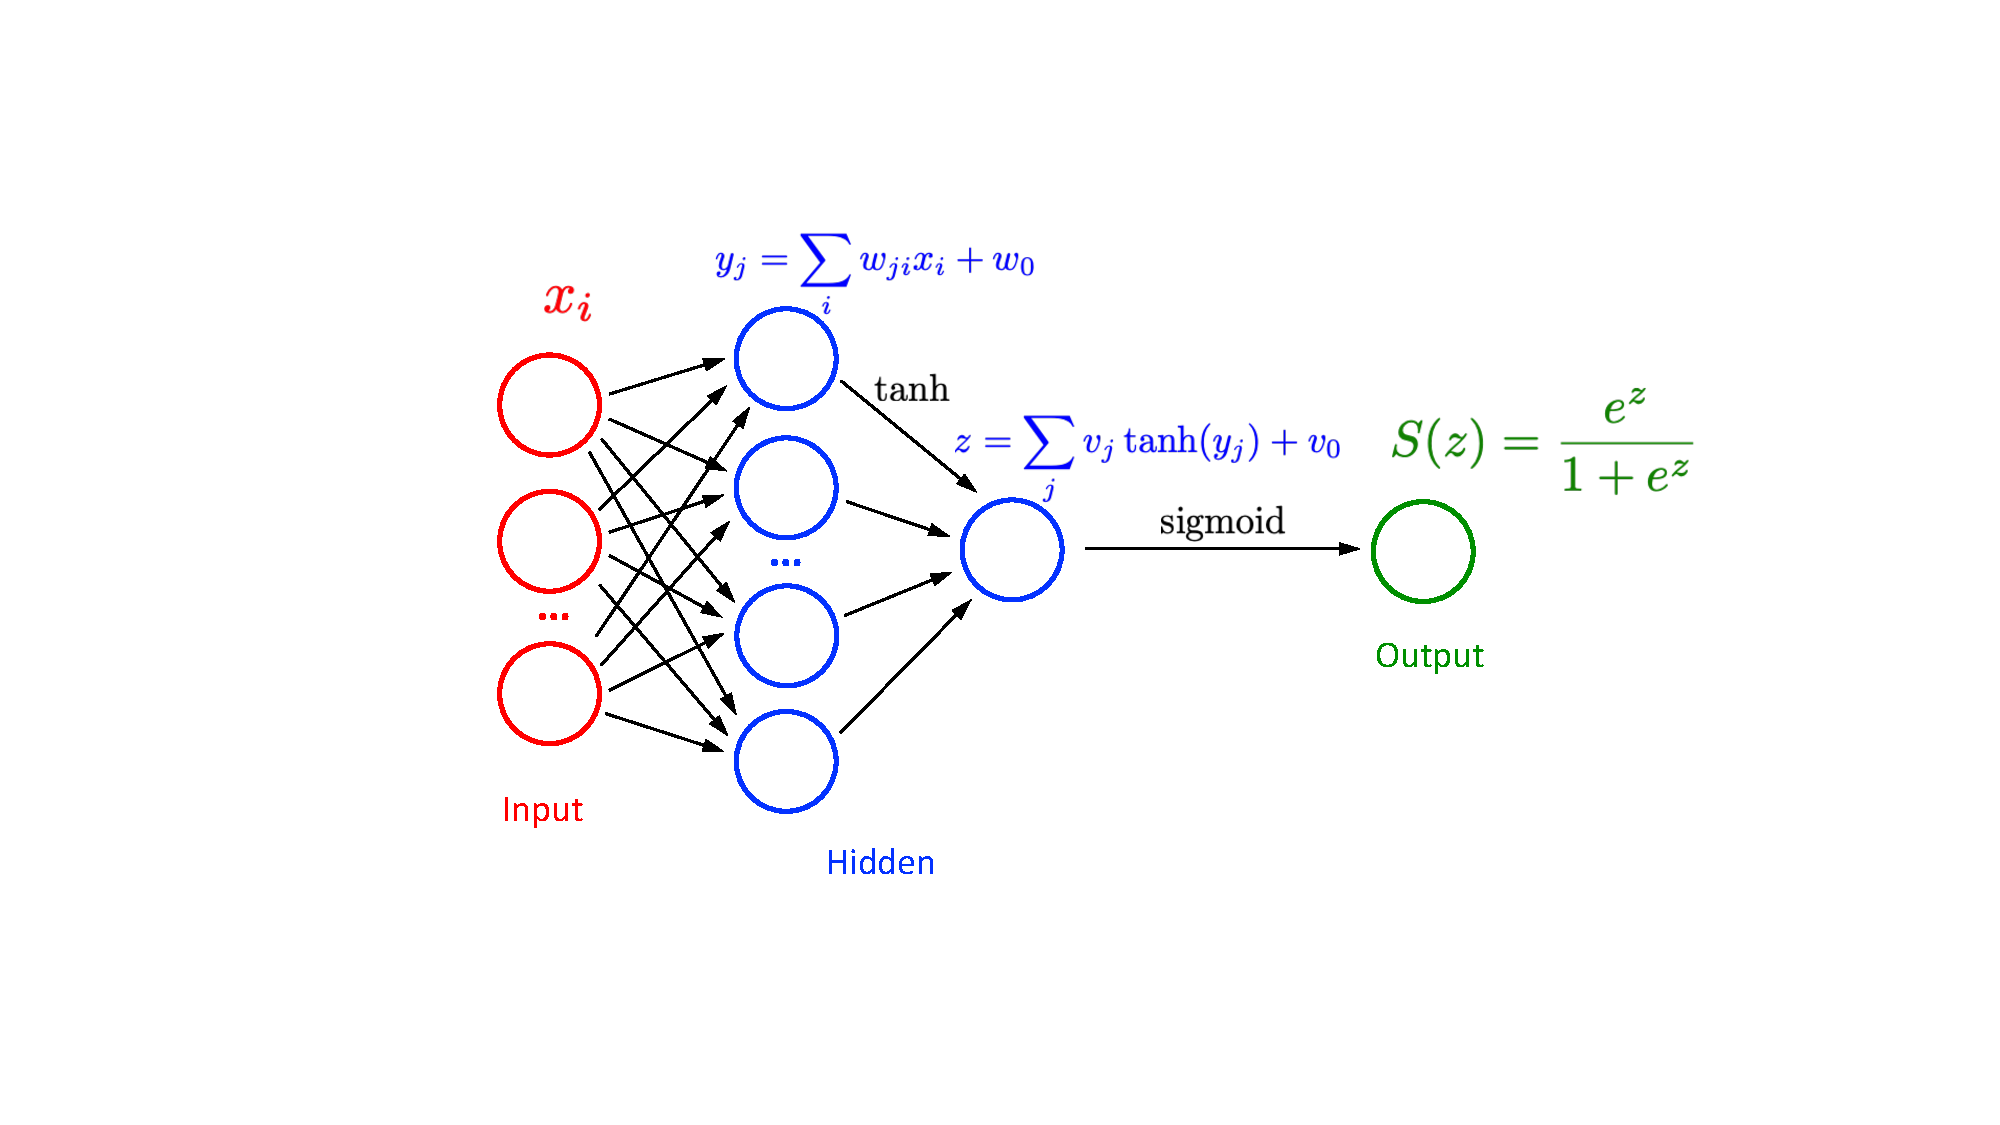
\includegraphics[width=0.45\textwidth]{plots/CNN_network.pdf}
\caption{
NN architecture that we use in the construction of the probabilistic catalogs.
The activation function in the output layer is sigmoid $S(x) = {e^{x}}/{(1 + e^{x})}$.
}
\label{fig:NN_structure}
\end{figure}

The general architecture of the NN that we use in this paper is shown in Fig. \ref{fig:NN_structure}.
It is a fully connected NN with 11 input nodes (shown by red circles with input features $x_i$), one hidden layer (shown by blue circles),
and an output layer (shown by the green circle).
The hidden layer consists of several nodes with values $y_j$. 
For the activation function at the hidden layer we use either hyperbolic tangent (tanh - shown on the plot) or rectified linear unit (relu).
The activation function for the output layer is sigmoid, which we use to make sure that the output value can be interpreted as a class probability.
The unknown parameters are weights of features in the hidden layer $w_{ji}$ and in the output layer $v_j$ including
offsets $w_{j0}$ and $v_0$.
The unknown parameters are optimized by minimizing a loss function, which we choose to be
the cross entropy
$-\text{log}L = - \sum_i (y_i\text{log}(p_i)+(1-y_i)\text{log}(1 - p_i))$, 
where $y_i = 0,\,1$ are the true labels of the sources and $p_i$ are the predicted class probabilities.
We have also used NN with two hidden layers, but the accuracy was similar to the networks with one hidden layer (Appendix \ref{sec:app}). For the final classification model, we have chosen to use one hidden layer.

\begin{figure}[h]
\centering
\hspace*{-0.5cm}
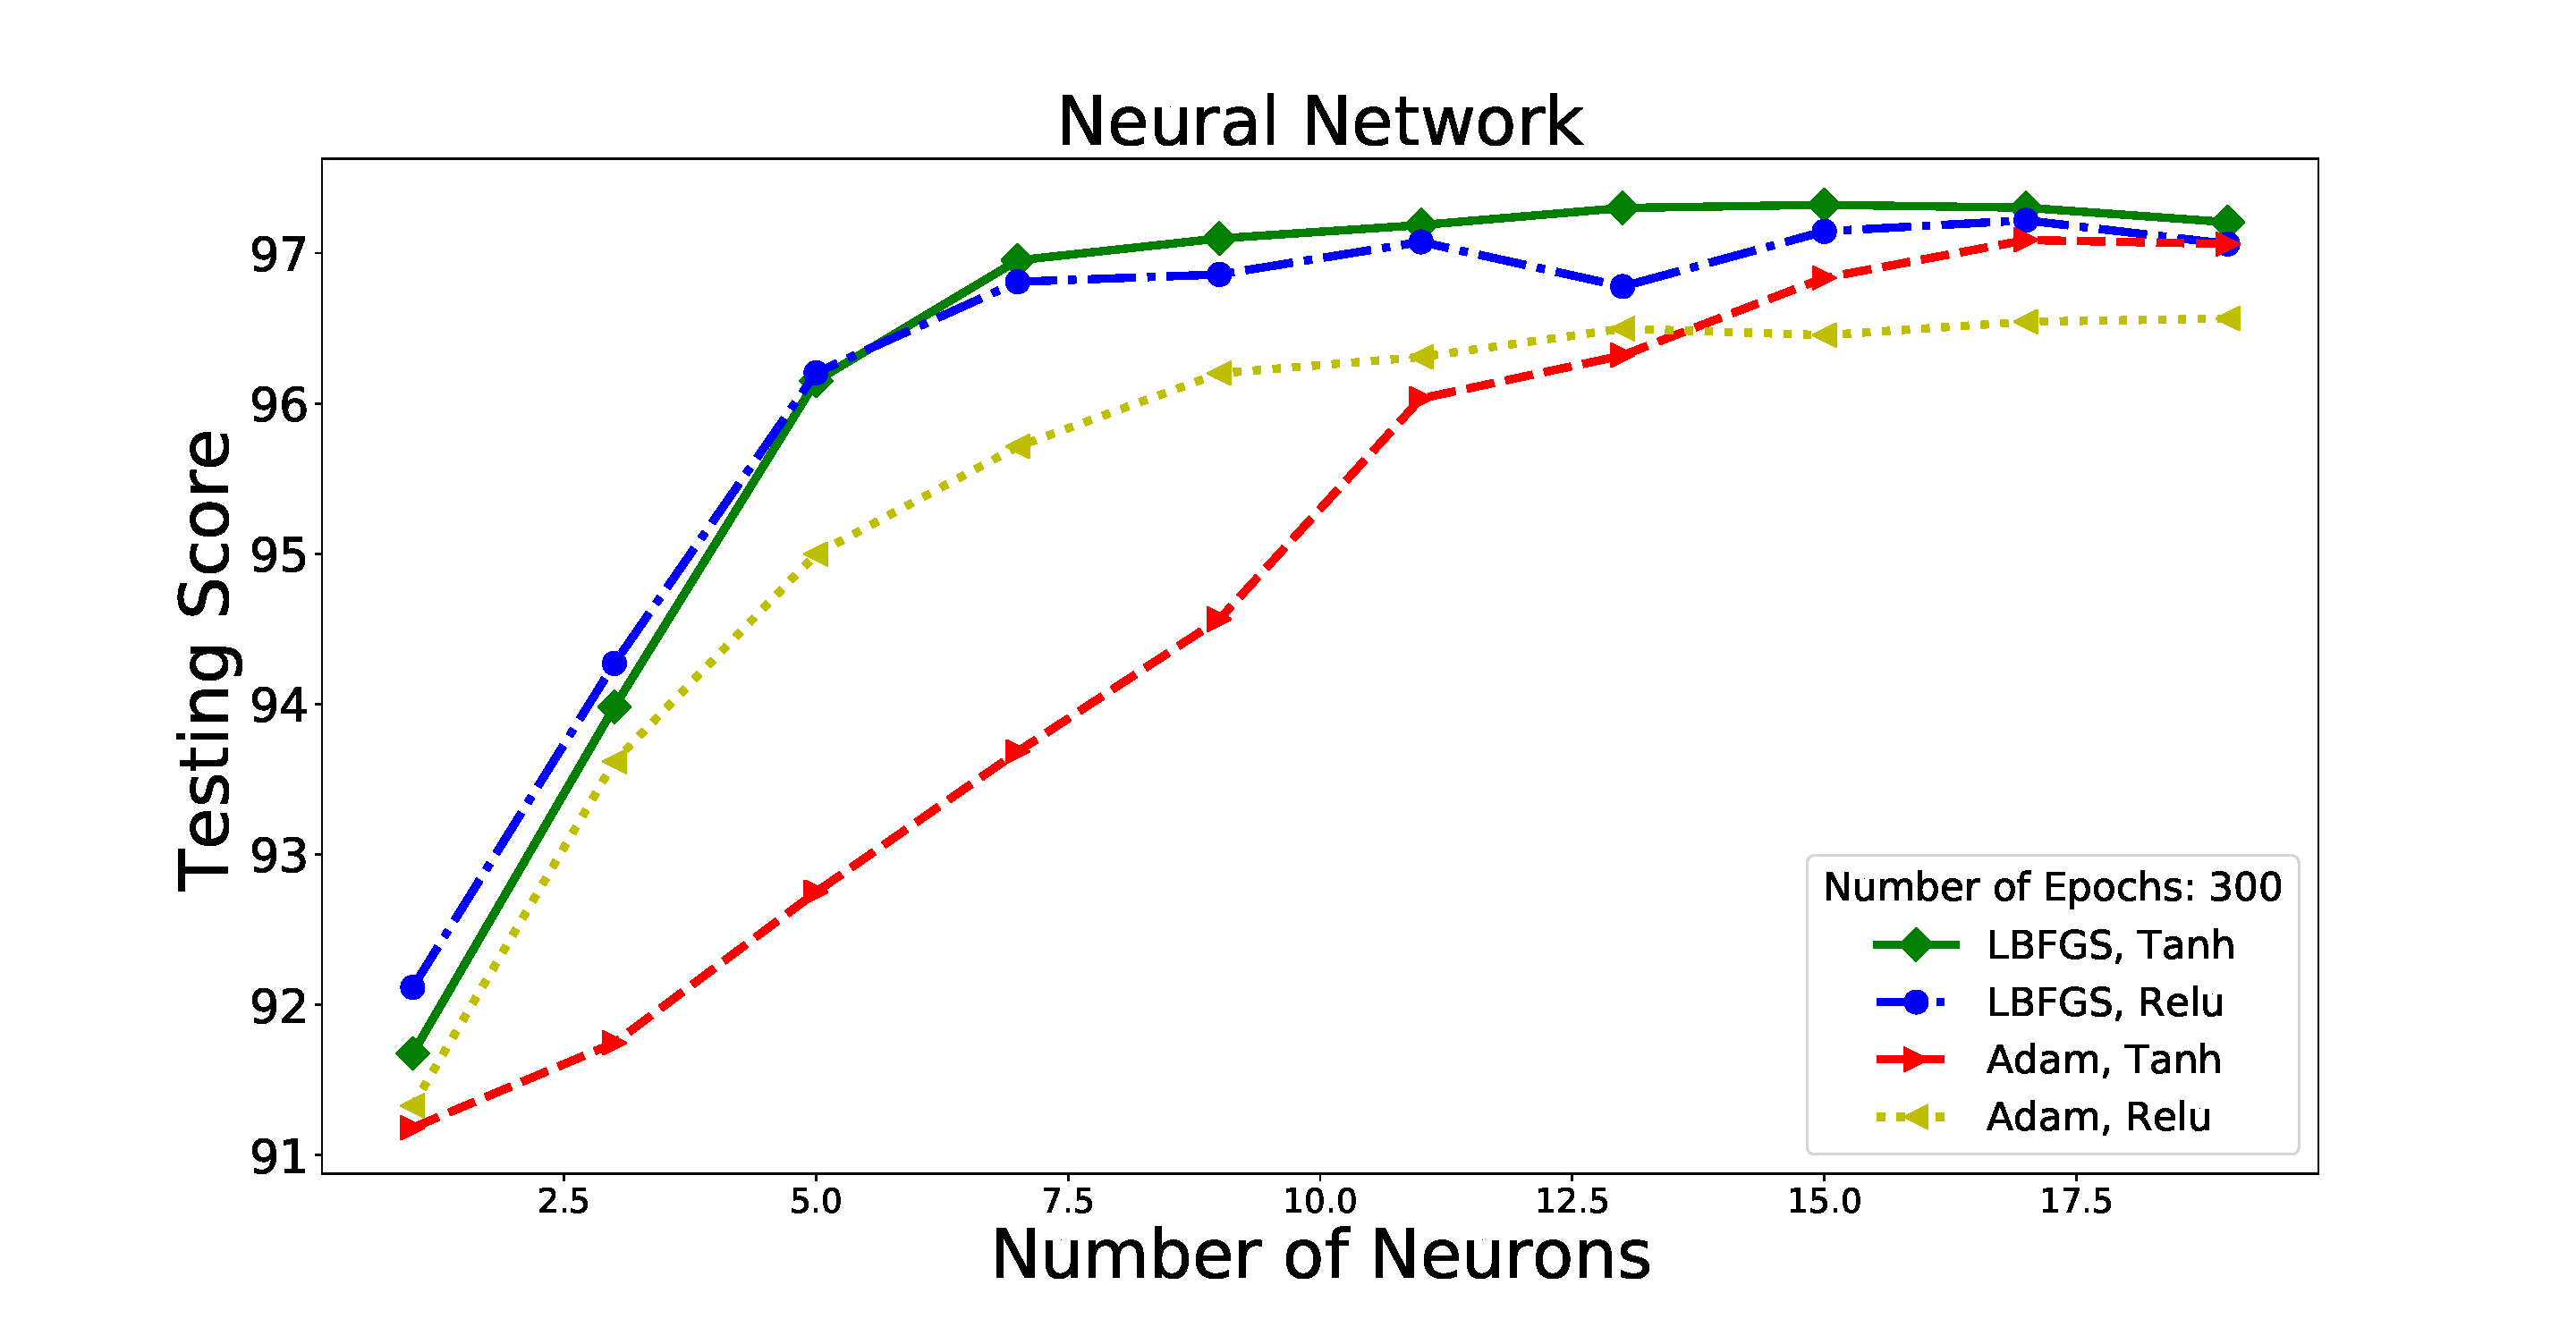
\includegraphics[width=0.5\textwidth]{plots/nn_train_neurons_assocnewfeat.pdf}
\caption{Dependence of accuracy on the number of neurons for different NN models.}
\label{fig:NN_neurons}
\end{figure}

Dependence of the testing accuracy on the number of neurons in the hidden layer, on the activation function, 
and on the optimization algorithm is shown in Fig. \ref{fig:NN_neurons}. 
We compare two activation functions at the hidden layer (tanh and relu) and two optimization algorithms: 
Limited memory Broyden-Fletcher-Goldfarb-Shanno \citep[LBFGS,][]{lbfgs} 
and the stochastic gradient descent algorithm Adam \citep{2014arXiv1412.6980K}.
We use 300 epochs for training.
Around 11 neurons in the hidden layer appears to be an optimal choice, since increasing the number of neurons leads to no significant increase in accuracy for all models. 

Dependence on the number of epochs (number of iterations in fitting) is presented in Fig. \ref{fig:NN_epochs}. 
The accuracy increases with higher number of epochs and saturates at around 200 for LBFGS and 300 for Adam. 




\begin{figure}[h]
\centering
\hspace*{-0.5cm}
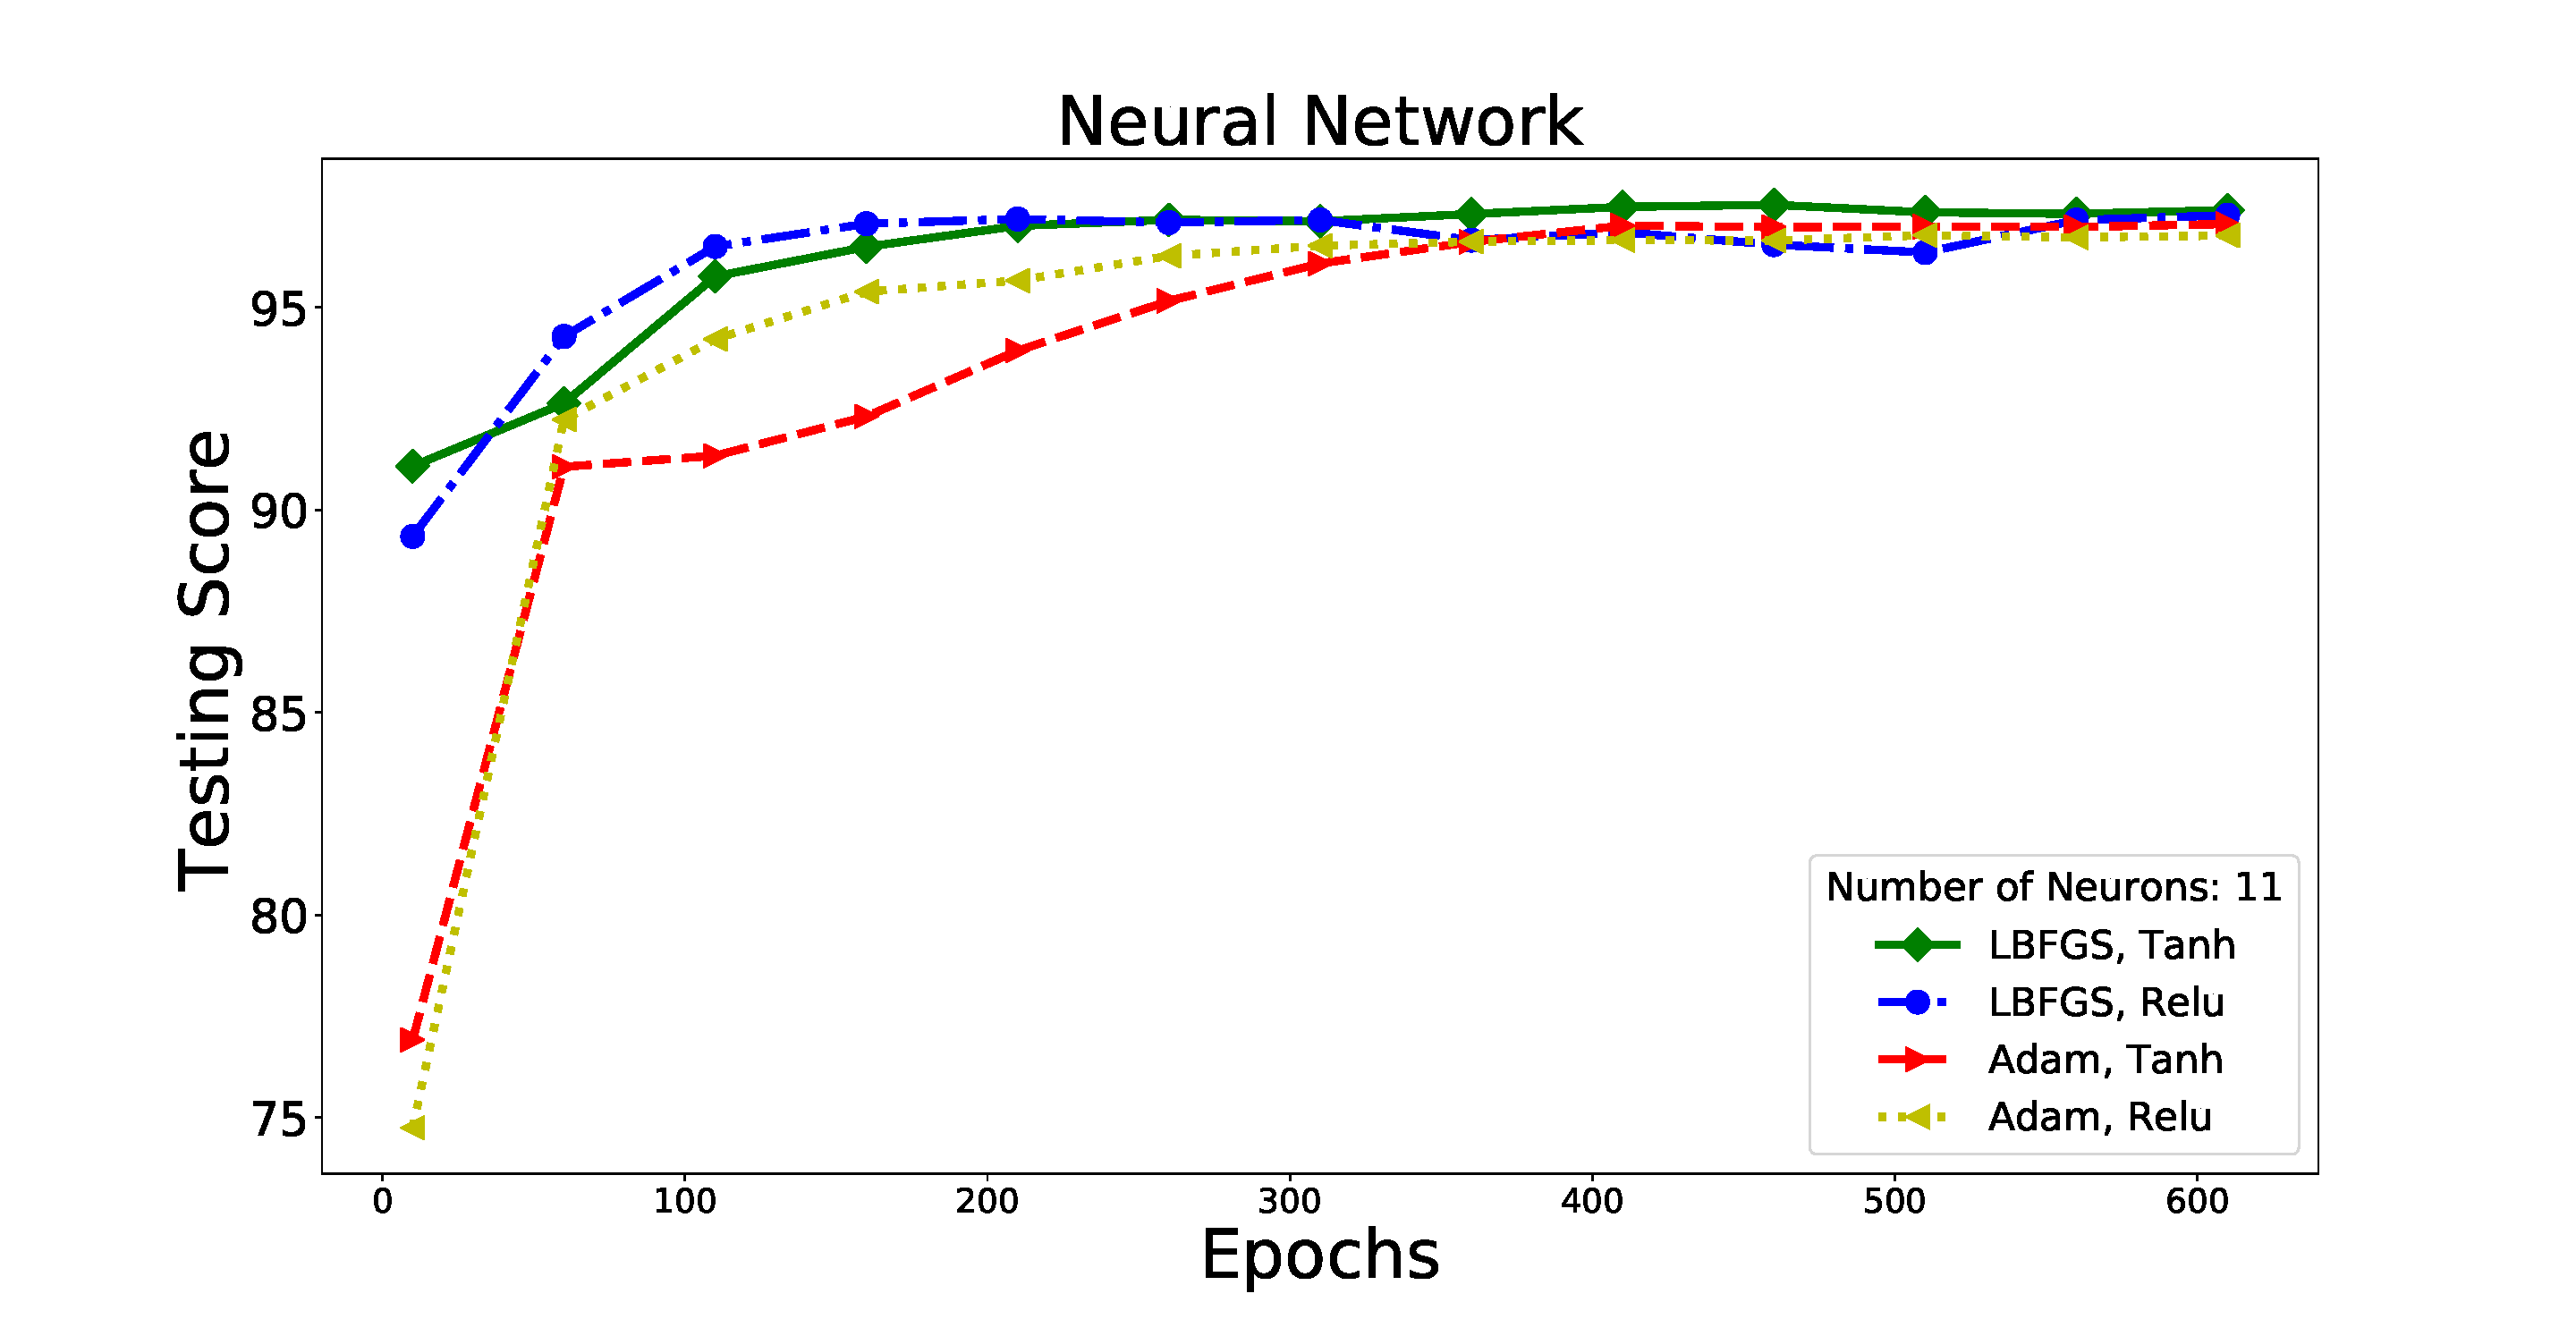
\includegraphics[width=0.5\textwidth]{plots/nn_train_epochs_assocnewfeat.pdf}
\caption{
Dependence of testing accuracy on the number of epochs in training for different solvers and activation functions.
}
\label{fig:NN_epochs}
\end{figure}
 
We illustrate the classification domains for NN with two input features in Fig. \ref{fig:NN_domains}. 
In this case we also use only two neurons in the hidden layer.
One can see that the separation boundary is smoother compared to the RF domains in Fig. \ref{fig:RF_domains} or BDT domains in Fig. \ref{fig:BDT_domains}.
For our final model we chose one hidden layer with eleven neurons, 300 training epochs, LBFGS solver, and tanh activation function at the hidden layer.


\begin{figure}[h]
\centering
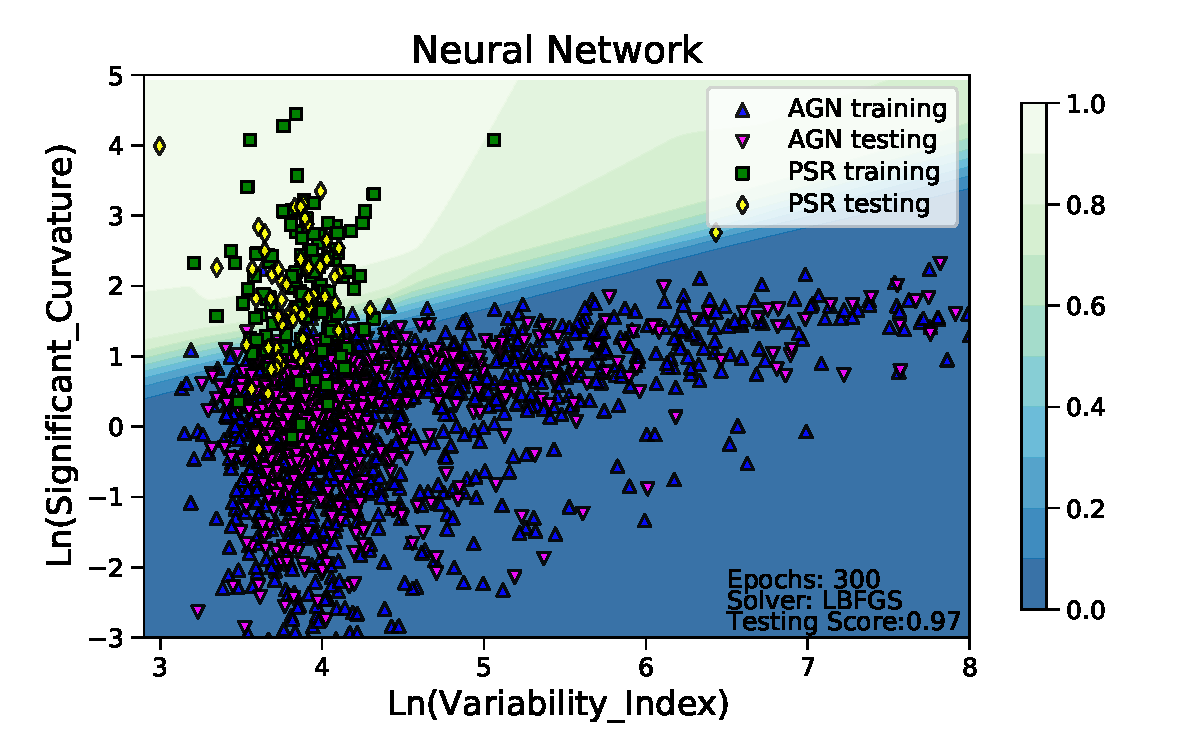
\includegraphics[width=0.5\textwidth]{plots/classification_domains/nn_300_lbfgs.pdf}
\caption{NN classification domains for 2 input features
averaged over 100 random splits into training and testing samples.
We use 2 neurons in the hidden layer. 
We use tanh activation function and LBFGS solver. 
}
\label{fig:NN_domains}
\end{figure}

\subsubsection{Logistic Regression}

As we have discussed in Section \ref{sec:class_alg}, 
the probability to belong to class 1 or 0 in LR is represented by the sigmoid function
$p_1(x) = 1 - p_0(x) = \frac{e^{m(x)}}{1 + e^{m(x)}}$ (see Eq. (\ref{eq:logit})),
where $m(x)$ is a function of input features $x$.
The complexity of the model is given by the number of parameters in $m(x)$.
We have considered two cases for $m(x)$: linear and quadratic function of the input features $x$.
Quadratic $m(x)$ resulted in a similar accuracy as linear $m(x)$.
Consequently, we have restricted our attention to linear functions $m(x) = f_0 + \sum_{k = 1}^{11} f_k x_k$.
In Fig. \ref{fig:LR_accuracy} we show the accuracy of the LR method as a function of the number of iterations
for different solvers, e.g., LBFGS \citep{lbfgs}, Stochastic Average Gradient \citep[SAG,][]{sag}, SAGA \citep[a variant of SAG,][]{saga},
and liblinear \citep[a special solver for LR and support vector machine classifications,][]{ll}.
As one can see from Fig. \ref{fig:LR_accuracy}, LBFGS and Liblinear outperform the other two solvers and converge much faster.
In order to illustrate the probability domains in LR, we show the classification with two features (LBFGs, 200 iterations)
in Fig. \ref{fig:LR_domains}. The domains look similar to the domains in the NN case (Fig. \ref{fig:NN_domains}).
For the final classification we will use LBFGs solver with 200 iterations.


\begin{figure}[h]
\centering
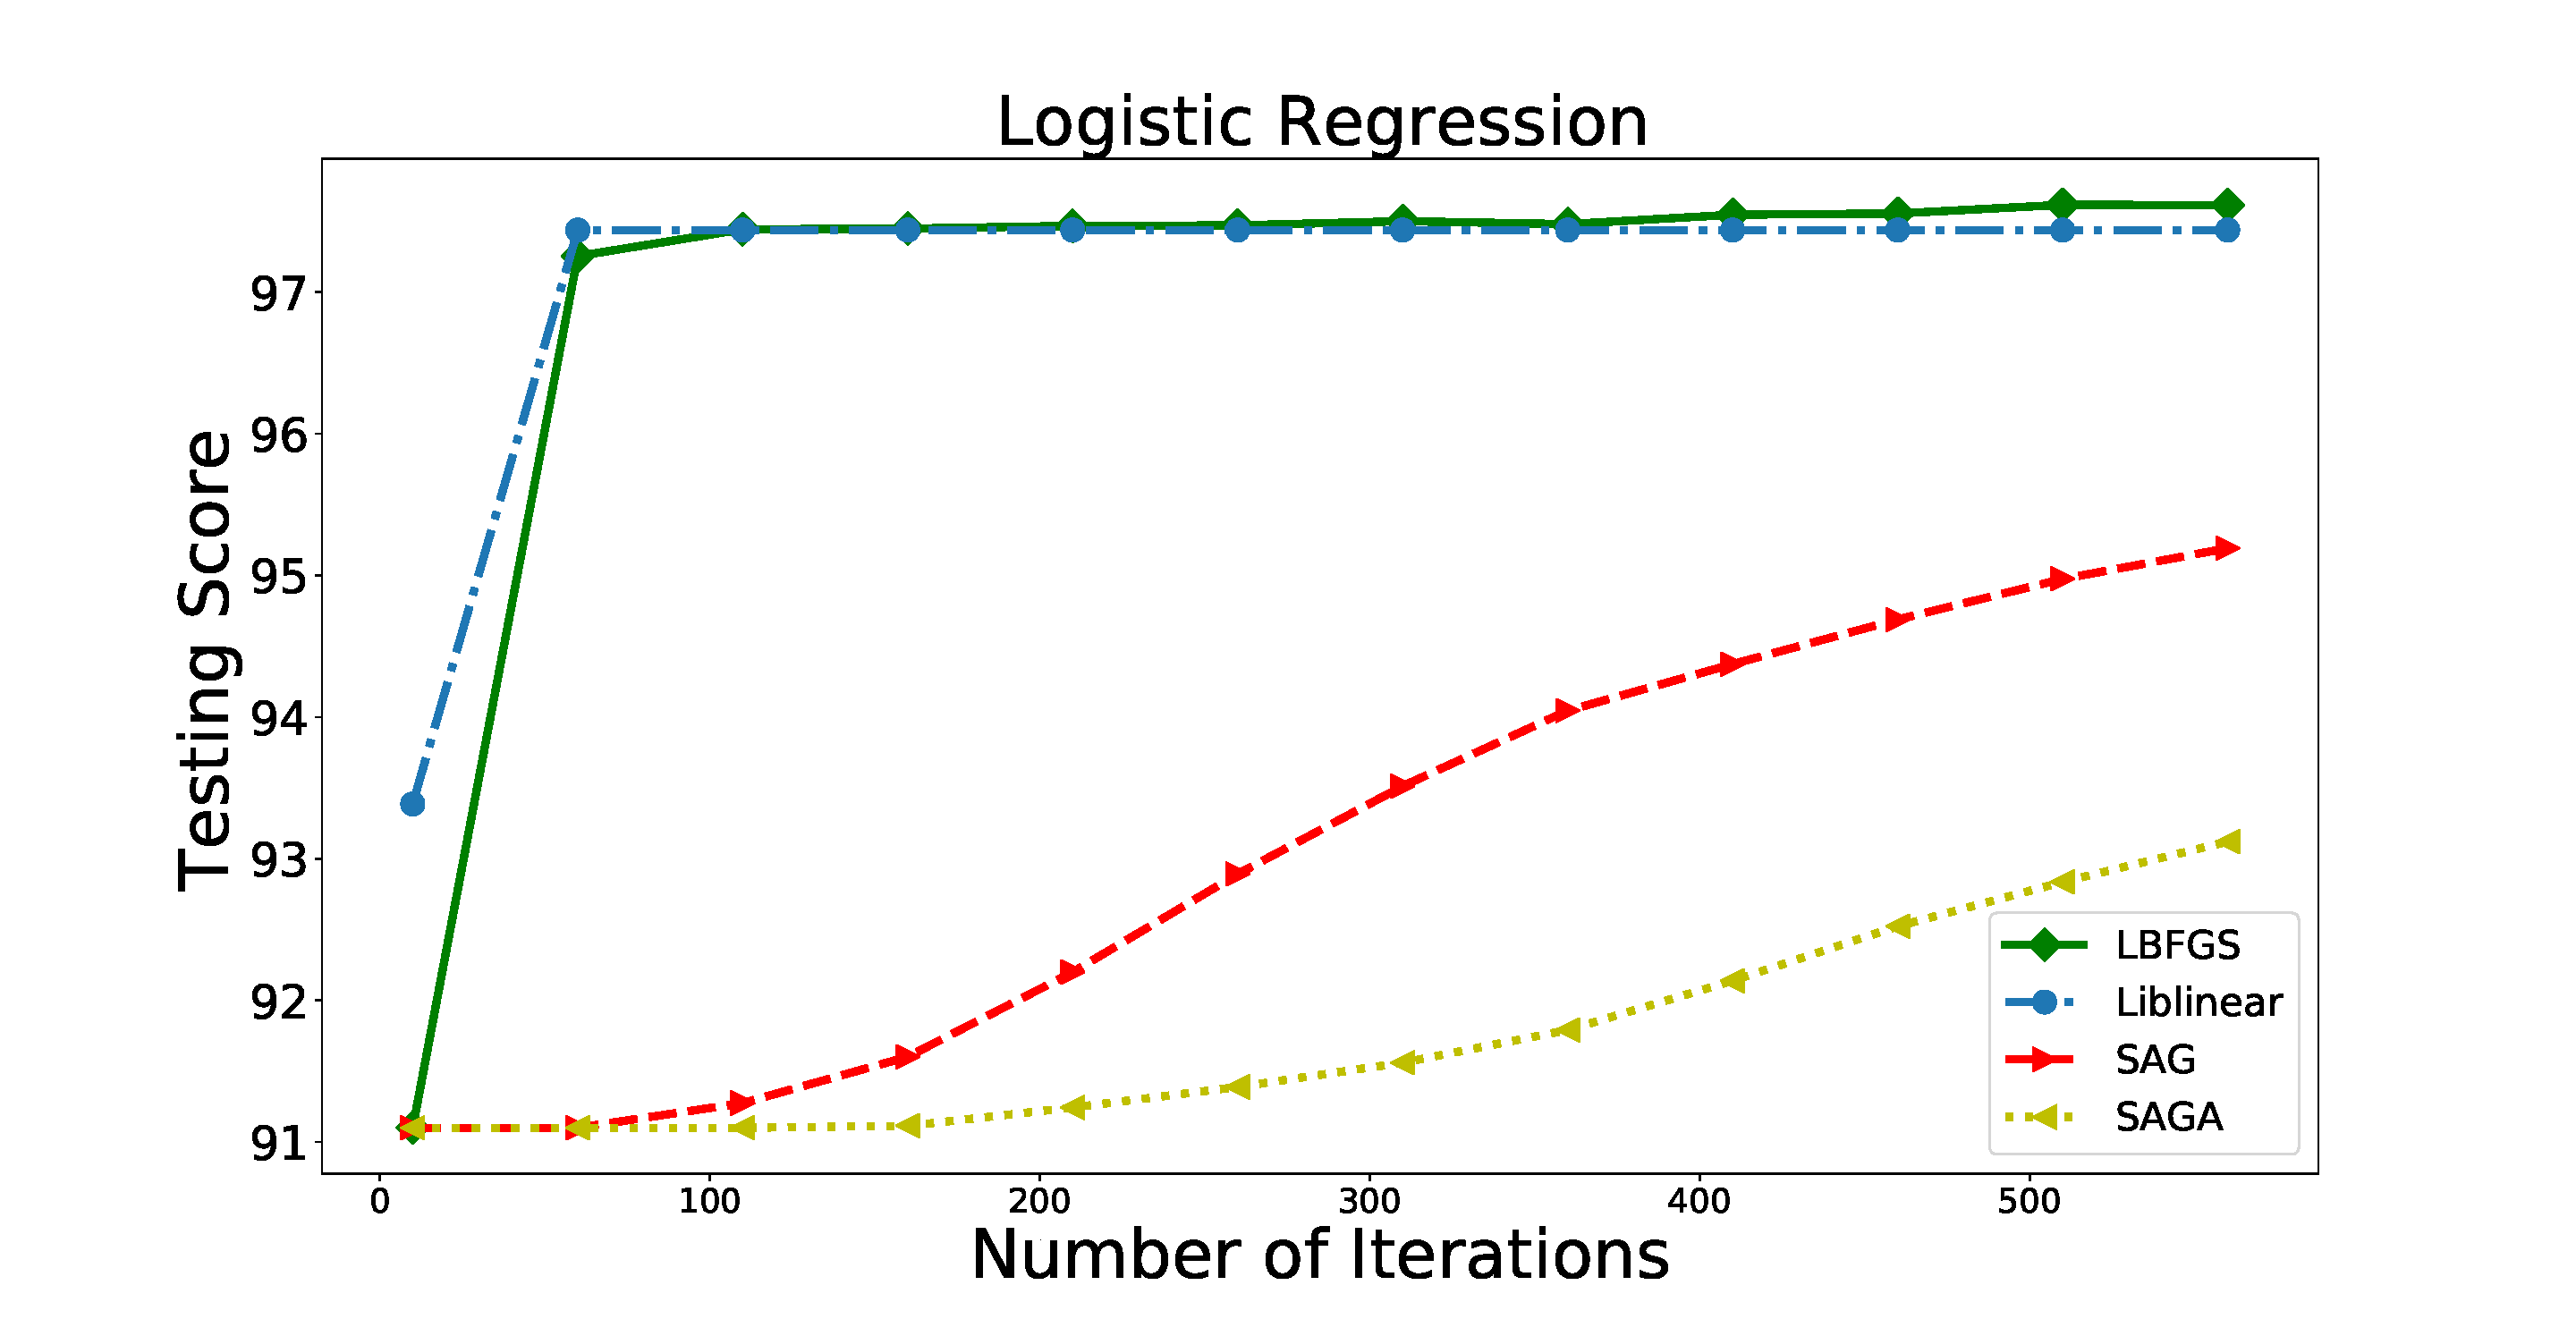
\includegraphics[width=\twopicsp\textwidth]{plots/lr_train_assocnewfeat.pdf}
\caption{Dependence of LR testing accuracy on the number of iterations for different solvers.}
\label{fig:LR_accuracy}
\end{figure}



\begin{figure}[h]
\centering
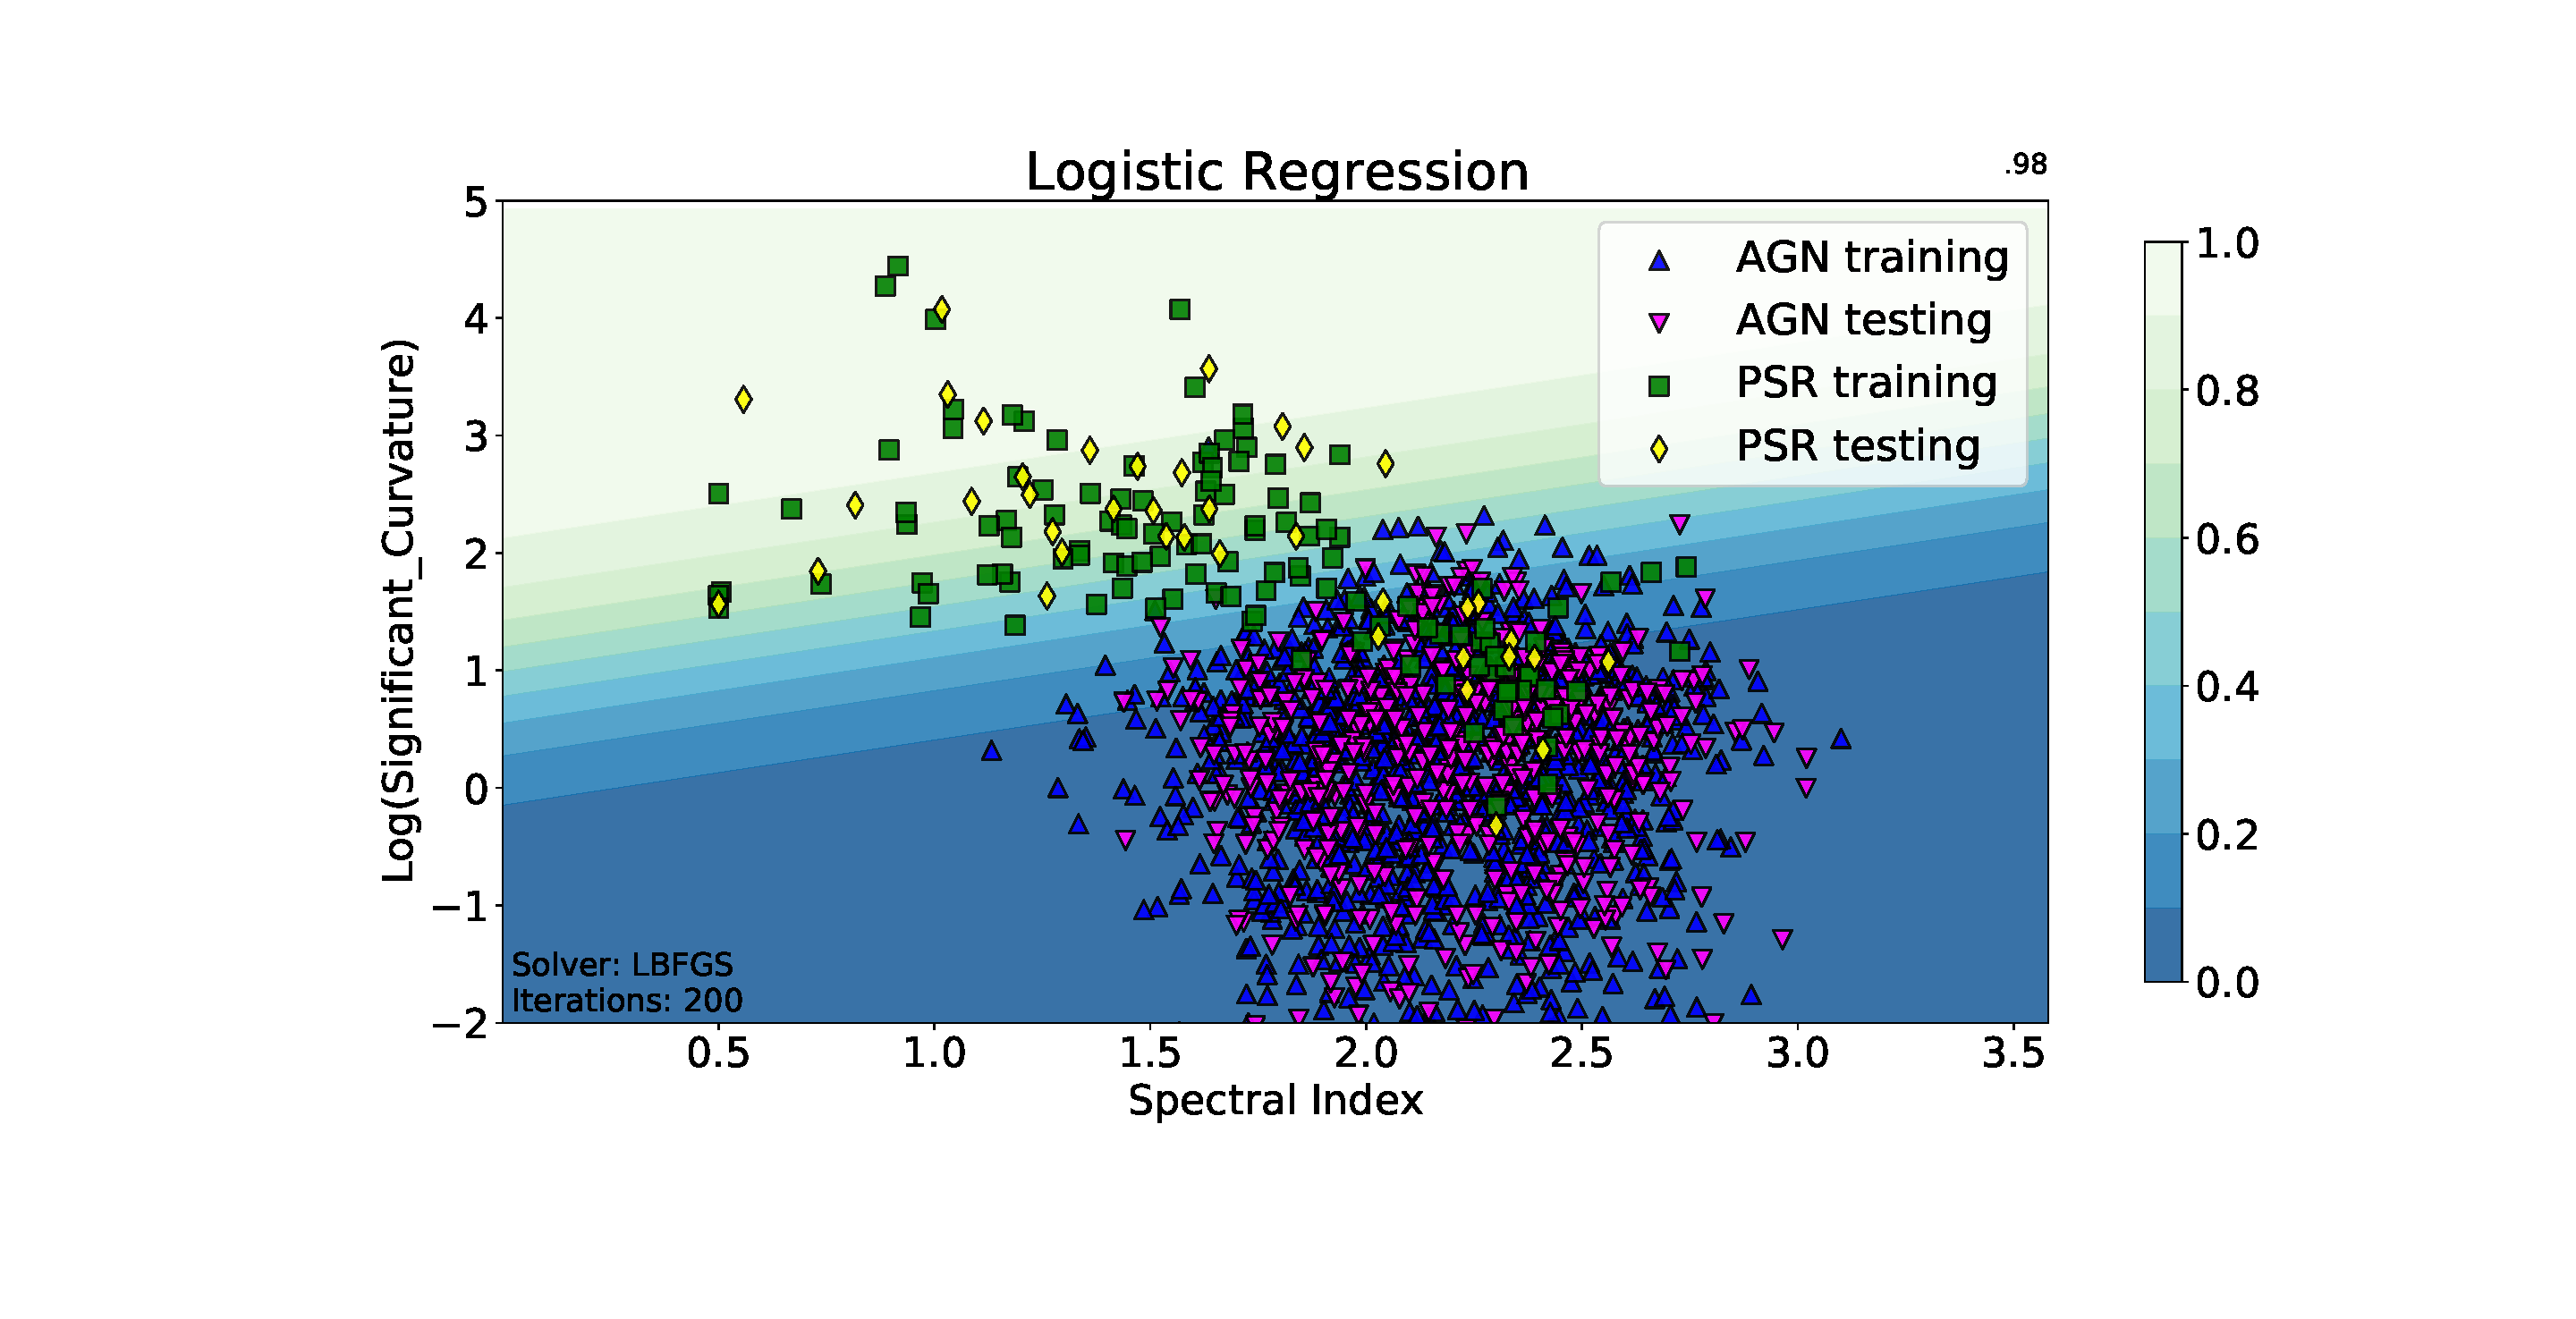
\includegraphics[width=0.5\textwidth]{plots/classification_domains/lr_200_lbfgs.pdf}
\caption{Classification domains for LR with two features 
averaged over 100 random splits into training and testing samples.}
\label{fig:LR_domains}
\end{figure}


\subsection{Oversampling}
\lb{sec:oversampling}

\Fermi-LAT catalogs have many more AGNs than pulsars, i.e., the datasets are imbalanced.
For example, the 3FGL catalog has 1744 associated AGNs (1739 without missing or unphysical values)
and 167 associated pulsars (166 without missing or unphysical values).
In the previous subsections we have optimized the overall accuracy. In this case, the algorithms try to identify AGNs rather than pulsars,
since it gives better accuracy. As a result, in the region of parameter space, where both pulsars and AGNs are present, the algorithms
will give higher probability for a source to be an AGN.


The problem of classification of imbalanced datasets can be quantitatively described in terms of precision and recall.
If we denote by ``\# true'' the number of pulsars in the dataset, by ``\# positive'' -- the number of sources predicted to be pulsars, and by 
``\# true positive'' -- the number of pulsars predicted to be pulsars, then  $precision \rm = \frac{\#\ true\ positive}{\#\ positive}$ is a measure how clean the prediction is, while $recall \rm = \frac{\#\ true\ positive}{\#\ true}$ is a measure how well the algorithm can detect the pulsars, i.e., how complete is the list of predicted pulsars.
If we reduce the pulsar domain by attributing uncertain sources predominantly to AGNs, then for pulsars the precision will increase, but the recall will decrease.



\begin{figure}[h]
\centering
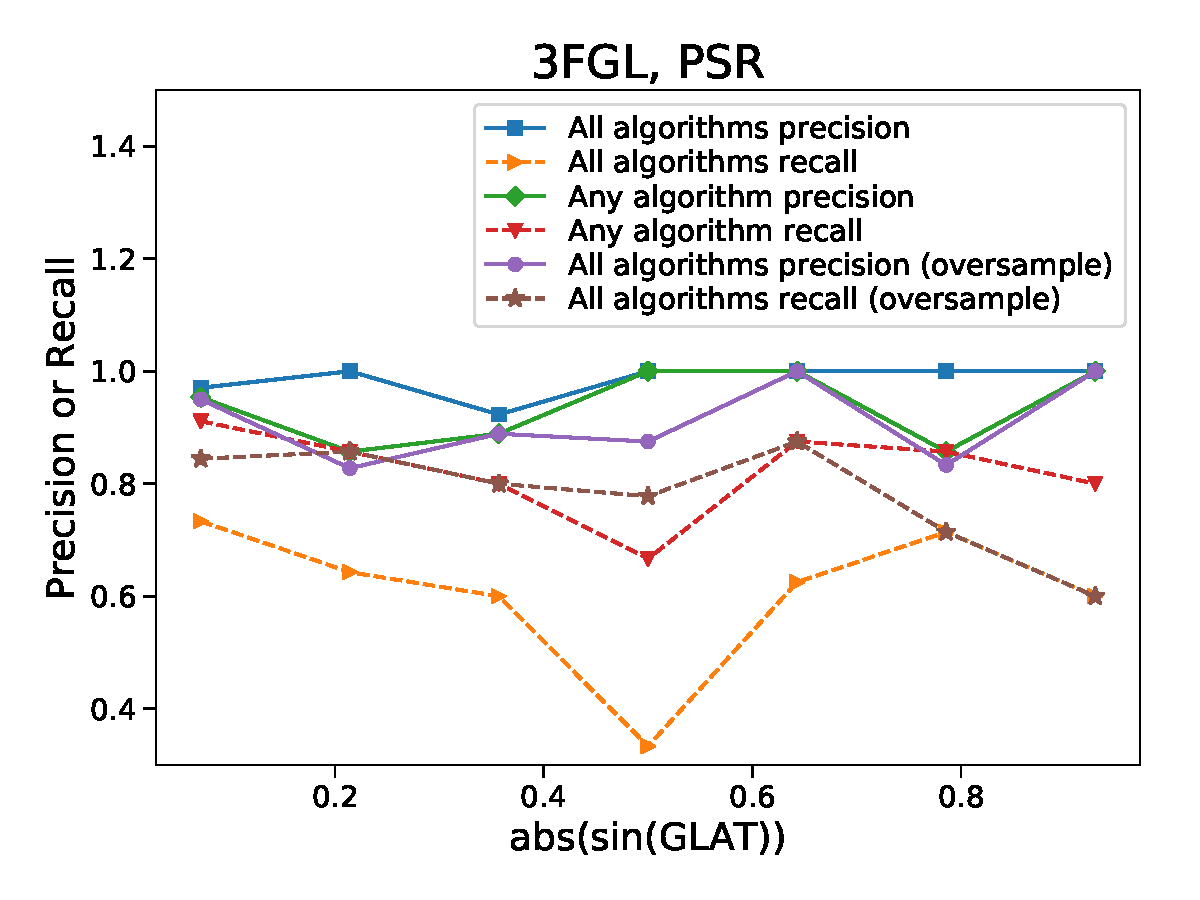
\includegraphics[width=\twopicsp\textwidth]{plots/all_algs_3FGL_precision_recall_oversample_PSR.pdf}
\caption{Precision and recall for pulsars using all-algorithm and any-algorithm classification for unweighted training data and
all-algorithm classification for oversampling of pulsars in training data. For details see Section \ref{sec:oversampling}.}
\label{fig:prec_recall}
\end{figure}


In Fig. \ref{fig:prec_recall} we show precision and recall for classification of pulsars.
In particular, in the first two lines (solid blue with squares and dashed orange with right triangles) a source is categorized as a pulsar if all four algorithms classify it as a pulsar,
while in lines 3 and 4 (solid green with diamonds and dashed red with down triangles) a source is attributed to the PSR class, if any of the algorithms classifies it as a pulsar.
It is clear that for lines 1 and 2 the pulsar domain is smaller than for lines 3 and 4, since in the former case, the domain is the intersection of domains for individual algorithms, while in the latter it is the union.
For all-algorithms classification the precision is 100\% for most of latitudes, while the recall is between 40\% and 80\%, i.e., the list of pulsars is generally clean but incomplete.
In case of any-algorithm classification, the recall is increased by about 20\% for most latitudes compared to the all-algorithms classification, but the precision drops by up to 20\% at some latitudes, i.e., the completeness improves at the expense of cleanliness of the sample.
Alternatively to using any-algorithm classification, one can give larger weights to pulsars or oversample pulsars in the training process, i.e., use the same source several times, so that the numbers of pulsars and AGNs in training are the same.
Provided that in some applications it is beneficial to have as complete as possible the list of pulsar candidates among unassociated sources, we have retrained the algorithms using oversampling with the same meta-parameters as in the previous sections.

In general one can either under- or oversample a dataset. Undersampling would reduce the number of AGNs to match the number of pulsars. However, since the total number of sources is not very high, we have chosen oversampling. 
For training with oversampling, we copy randomly existing pulsars and add them to the dataset until the number of pulsars and AGNs are the same.
Although pulsars in the training dataset are redundant, they help to increase the weight of pulsars in the classification model.
We illustrate the oversampling procedure in Fig. \ref{fig:LR_domains_O} top panel:
the number of times a source appears in training is shown by adding markers with shifts to the right and above the original position of the source (note that the shift is introduced for presentation only, the parameters of the sources are exactly the same as in the original source).
In the bottom panel of Fig. \ref{fig:LR_domains_O} we repeat Fig.  \ref{fig:LR_domains} in order to compare the classification domains with and without oversampling.
One can see that pulsar domain in the top panel is larger than the pulsar domain in the bottom panel.
As a result, in the top panel more pulsars are classified as pulsars but also more AGNs are falsely classified as pulsars in the intersection region. 
Since the overall number of AGNs is larger than the number of pulsars, the testing accuracy with oversampling is smaller than without oversampling.

The results of training with oversampling are presented  in Fig. \ref{fig:prec_recall},
lines 5 and 6 (solid purple with circles and dashed brown with stars). 
These lines show precision and recall when a source is categorized as a pulsar, if all four algorithms trained with oversampling classify it as a pulsar. 
The precision and recall in this case are similar to the any-algorithm classification for the training without oversampling.


\begin{figure}[h]
\centering

\includegraphics[width=0.5\textwidth]{plots/classification_domains/lr_200_lbfgs_oversample.pdf} \\
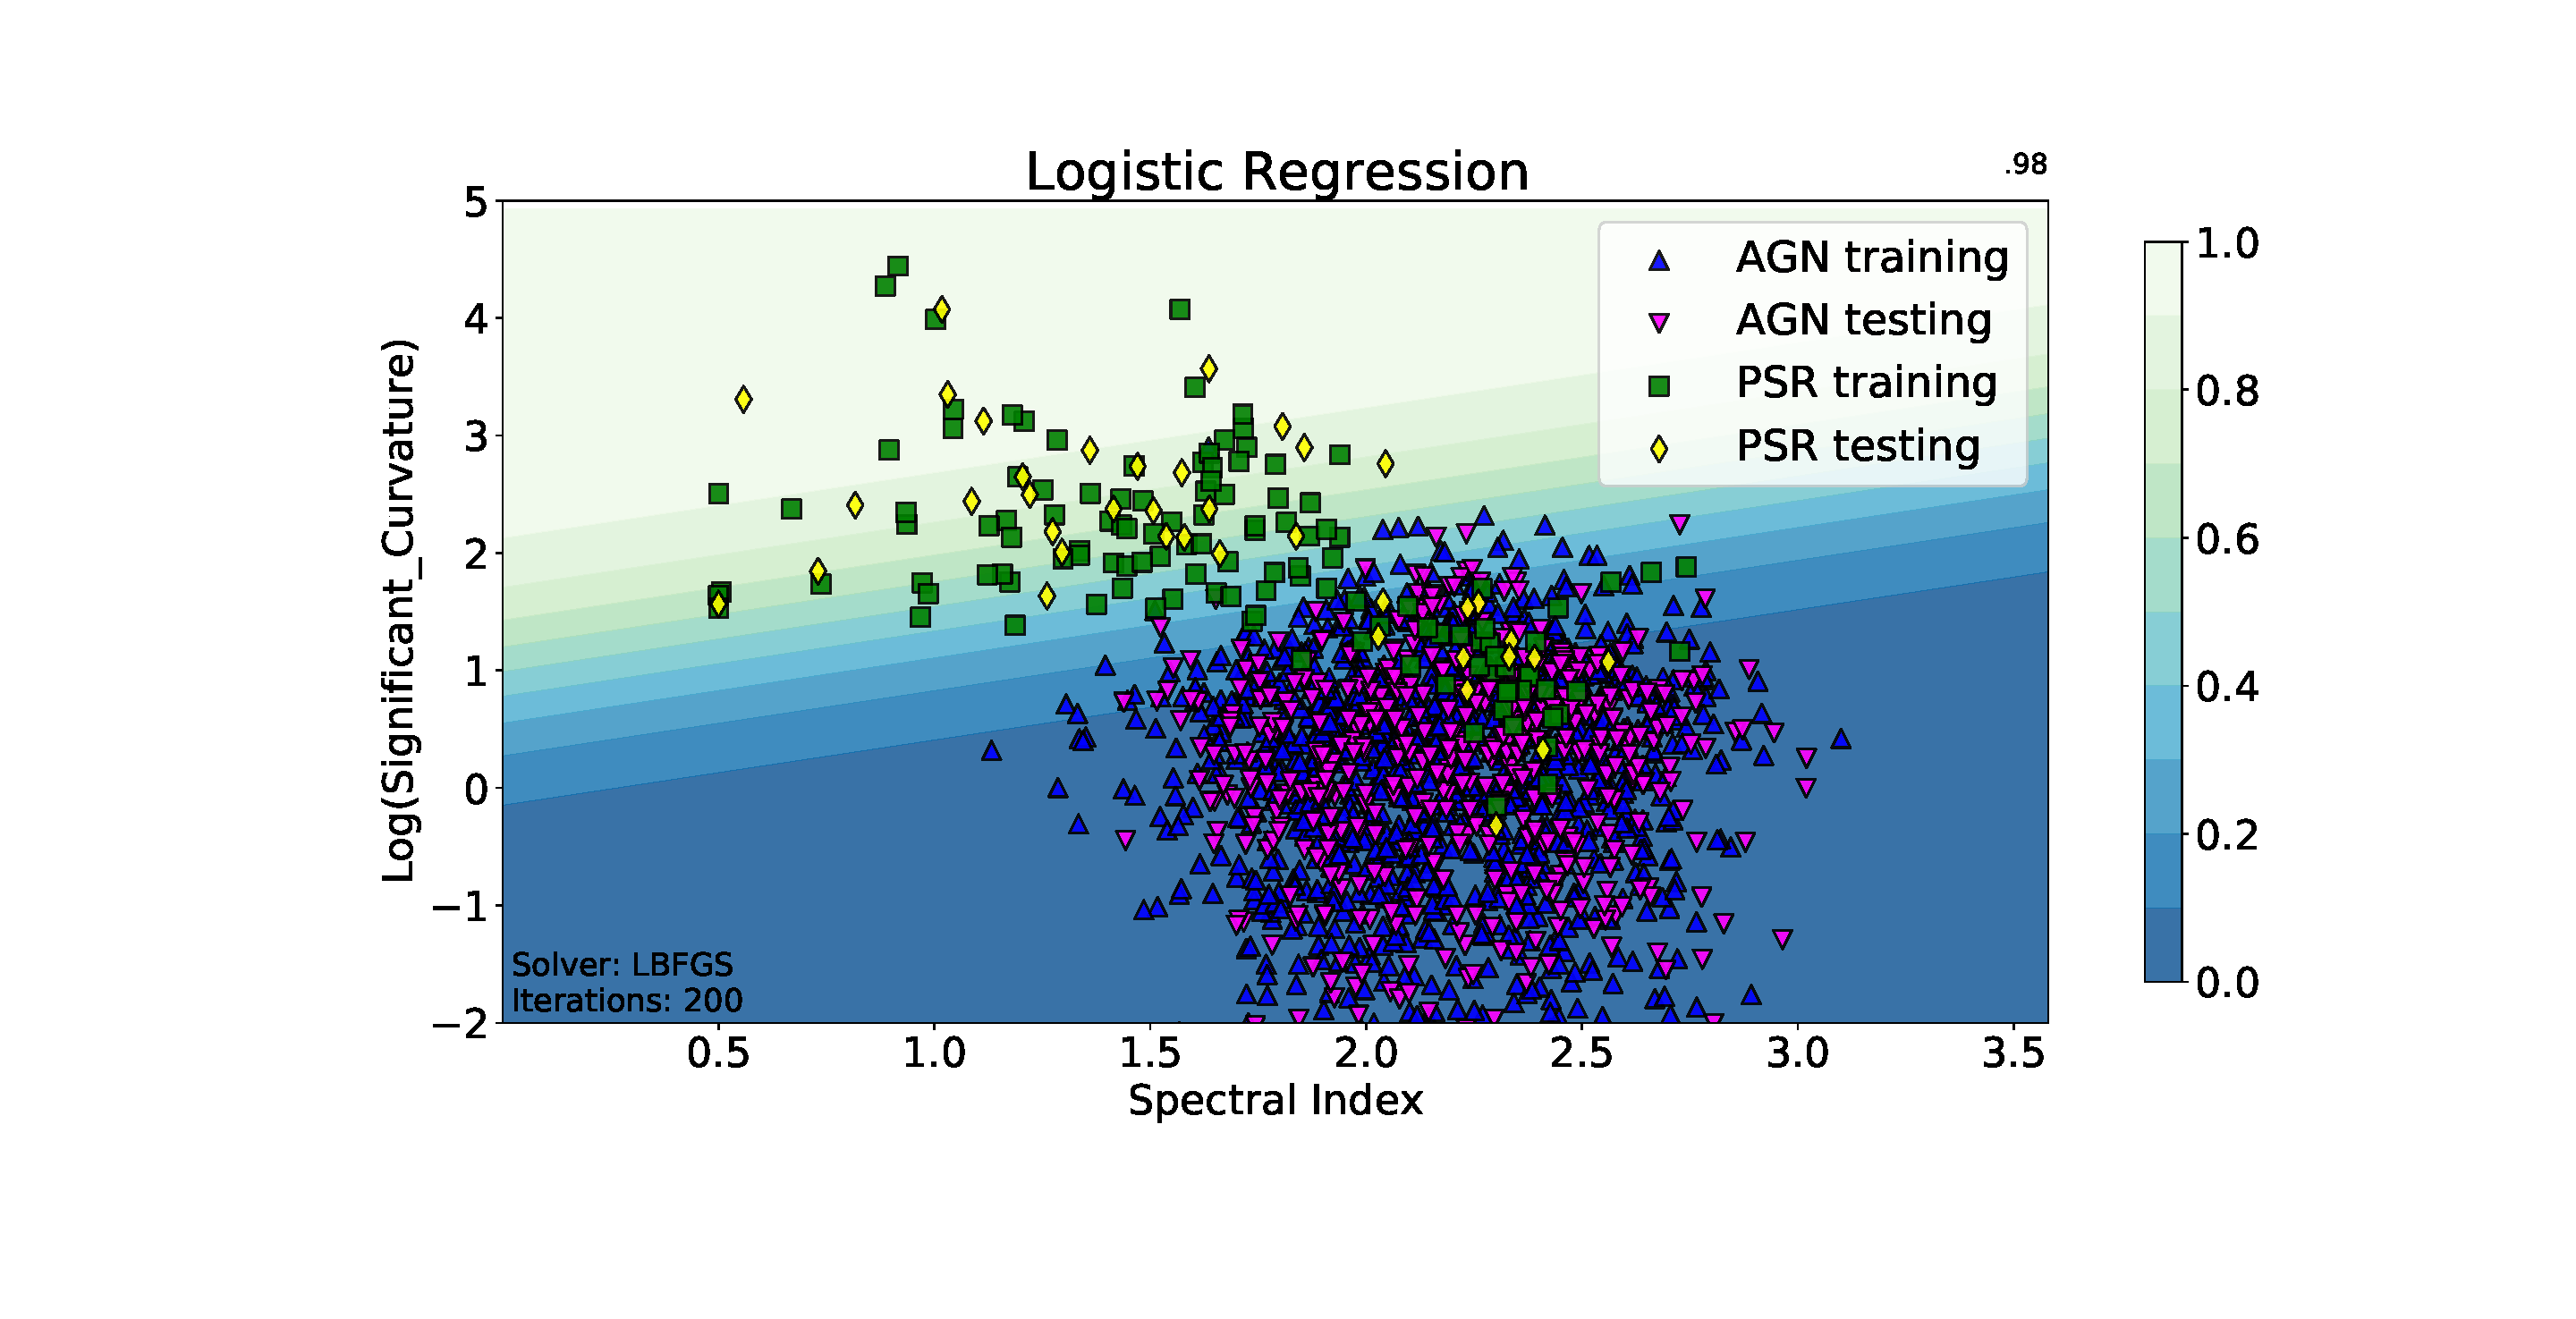
\includegraphics[width=0.5\textwidth]{plots/classification_domains/lr_200_lbfgs.pdf}
\caption{Top panel: LR classification domains showing class probabilities for training with oversampling.
The oversampling is illustrated by repeating the pulsar markers with a shift: the number of markers is equal to the number of times the pulsar appears in training.
Bottom panel: we repeat Fig. \ref{fig:LR_domains} for convenience of comparison with the oversampled training in the top panel.
In both panels the domains are obtained by averaging over 100 random splits into training and testing samples.
}  
\label{fig:LR_domains_O}
\end{figure}
